\documentclass[conference]{IEEEtran}

\usepackage[utf8]{inputenc}
\usepackage[T1]{fontenc}
\usepackage{amsmath,amssymb,amsfonts}
\usepackage{graphicx}
\usepackage{booktabs}
\usepackage{array}
\usepackage{hyperref}
\usepackage{xcolor}
\usepackage{fancyhdr}

% Auto-generated stamp definitions for CS-370 AI OEL
\newcommand{\stampline}{Muhammad Waleed Ahmed (513303) | Ahmad Raza (522356) | Ali Hamza (514549)}

% Auto-generated report numbers | Muhammad Waleed Ahmed (513303) | Ahmad Raza (522356) | Ali Hamza (514549)
% Do not edit manually; regenerate via python -m delivery.experiments.numbers
\newcommand{\numMNineAblationFullOwnExp}{892.2}
\newcommand{\numMNineAblationMstOnlyExp}{895.7}
\newcommand{\numPartaReflexScenarios}{30}
\newcommand{\numPartaReflexSuccessPct}{3.3}
\newcommand{\numPartaReflexSuccesses}{1}
\newcommand{\numPartbBTwoMeanExp}{3349.9}
\newcommand{\numPartbOwnMeanCost}{218.07}
\newcommand{\numPartbOwnMeanExp}{387.4}
\newcommand{\numPartbScenarios}{30}
\newcommand{\numPartbUcsMeanExp}{12299.6}
\newcommand{\numPartcDefaultMeanCost}{417.3}
\newcommand{\numPartcGamesCount}{50}
\newcommand{\numPartcPruningDSixOwnEvals}{137.4}
\newcommand{\numPartcPruningDSixSavedMmPct}{89.7}
\newcommand{\numPartcPruningPositions}{210}
\newcommand{\numPartcTunedMeanCost}{407.9}
\newcommand{\numPartcTunedWinPct}{42.0}
\newcommand{\numPartdNovalSuccessPct}{65.0}
\newcommand{\numPartdRequests}{20}
\newcommand{\numPartdWithvalSuccessPct}{70.0}


\pagestyle{fancy}
\fancyhf{}
\fancyhead[C]{\footnotesize \stampline}
\fancyfoot[C]{\footnotesize \thepage}
\renewcommand{\headrulewidth}{0pt}

\graphicspath{{figures/}}

\begin{document}

\title{Autonomous Delivery Agent Under Uncertainty, Dynamic Twists, and Adversarial Competition}

\author{
\IEEEauthorblockN{Muhammad Waleed Ahmed (513303), Ahmad Raza (522356), Ali Hamza (514549)}
\IEEEauthorblockA{Department of Computer Science, CS-370 Artificial Intelligence (Fall 2026)}
}

\maketitle
\thispagestyle{fancy}

\begin{abstract}
We design, implement, and empirically evaluate an autonomous grid-city delivery agent operating under heterogeneous terrain costs, stochastic movement slip ($p=0.23$), dynamic environment twists (\texttt{fog\_partial\_observability}, \texttt{one\_way\_streets}, and \texttt{fragile\_parcel}), an adversarial \texttt{chaser} rival, and a natural-language Large Language Model (LLM) dispatcher. All classical search (BFS, UCS, DLS, IDS, Greedy Best-First, A*), adversarial search (Minimax, Alpha-Beta with move ordering), and simulation components are implemented from scratch in Python and NumPy without external solver libraries. Across \numPartbScenarios{} certified scenarios, our admissible \texttt{CombinedMSTHeuristic} reduces A* node expansions by $96.8\%$ compared to UCS (\numPartbOwnMeanExp{} vs.\ \numPartbUcsMeanExp{}). At depth $6$, Alpha-Beta with custom move ordering prunes \numPartcPruningDSixSavedMmPct{}\% of Minimax evaluations across \numPartcPruningPositions{} positions. Finally, pre-execution argument validation raises live LLM dispatcher success from \numPartdNovalSuccessPct{}\% to \numPartdWithvalSuccessPct{}\% across \numPartdRequests{} benchmark requests.
\end{abstract}

\begin{IEEEkeywords}
Autonomous Agent, A* Search, Admissible Heuristics, Alpha-Beta Pruning, ReAct, Stochastic Simulation
\end{IEEEkeywords}

\section{Introduction, Instance, and Twists}
Autonomous last-mile delivery in urban grids requires combining optimal multi-stop route planning, real-time adaptation to stochastic execution errors, tactical evasion of competing agents, and safe natural-language tasking. Following the CS-370 Open Ended Lab (OEL) specification, we generate our canonical problem instance deterministically from the group CMS IDs \texttt{513303}, \texttt{514549}, and \texttt{522356} using the unmodified instructor script \texttt{oel\_instance.py}.

\subsection{Canonical Instance and Source Discrepancy (D14)}
The generated city (\texttt{432382d9}, Fig.~\ref{fig:canonical_grid}) is a $22 \times 22$ grid ($484$ cells) with obstacle density $0.269$ ($-1$ blocked cells) and strictly positive terrain entry costs $\{3, 4, 5, 7\}$ corresponding to \texttt{road}, \texttt{grass}, \texttt{mud}, and \texttt{ford}. The depot is located at $(4, 20)$, with $5$ delivery stops at $(5,15)$, $(16,1)$, $(15,12)$, $(9,7)$, and $(6,10)$. The assigned adversary is \texttt{chaser} with search depth $6$ plies, and the simulator slip probability is $p = 0.23$.

\textbf{Brief vs.\ Script Discrepancy (D14):} While the four-page assignment brief states $4$--$6$ delivery stops, the unmodified \texttt{oel\_instance.py} script samples $3$--$6$ stops (\texttt{1 + rng.integers(3, 7)} picks minus the start cell). Our codebase supports the full $3$--$6$ range without modifying the generator; our canonical instance contains $5$ stops.

\subsection{Dynamic City Twists}
Three twists modify the underlying state space, action legality, and transition model (not merely UI rendering):
\begin{enumerate}
    \item \texttt{fog\_partial\_observability} (assigned): Only cells within Chebyshev percept radius $\rho$ around the agent are observed; unseen cells use an optimistic minimum-cost prior in the planner's belief map, triggering replanning whenever newly revealed obstacles or higher-cost terrain invalidate the active plan (Fig.~\ref{fig:twist_fog}).
    \item \texttt{one\_way\_streets} (assigned): A deterministic fraction of adjacent edges are restricted to one-way traversal, repaired via strongly connected component (SCC) checks so all stops remain mutually reachable from the depot (Fig.~\ref{fig:twist_oneway}).
    \item \texttt{fragile\_parcel} (approved third twist): While the fragile parcel remains undelivered (tracked via the delivered bitmask), entering \texttt{mud} or \texttt{ford} cells is illegal, with the fragile destination cell exempted if needed to preserve solvability (Fig.~\ref{fig:twist_fragile}).
\end{enumerate}

\begin{figure}[t]
    \centering
    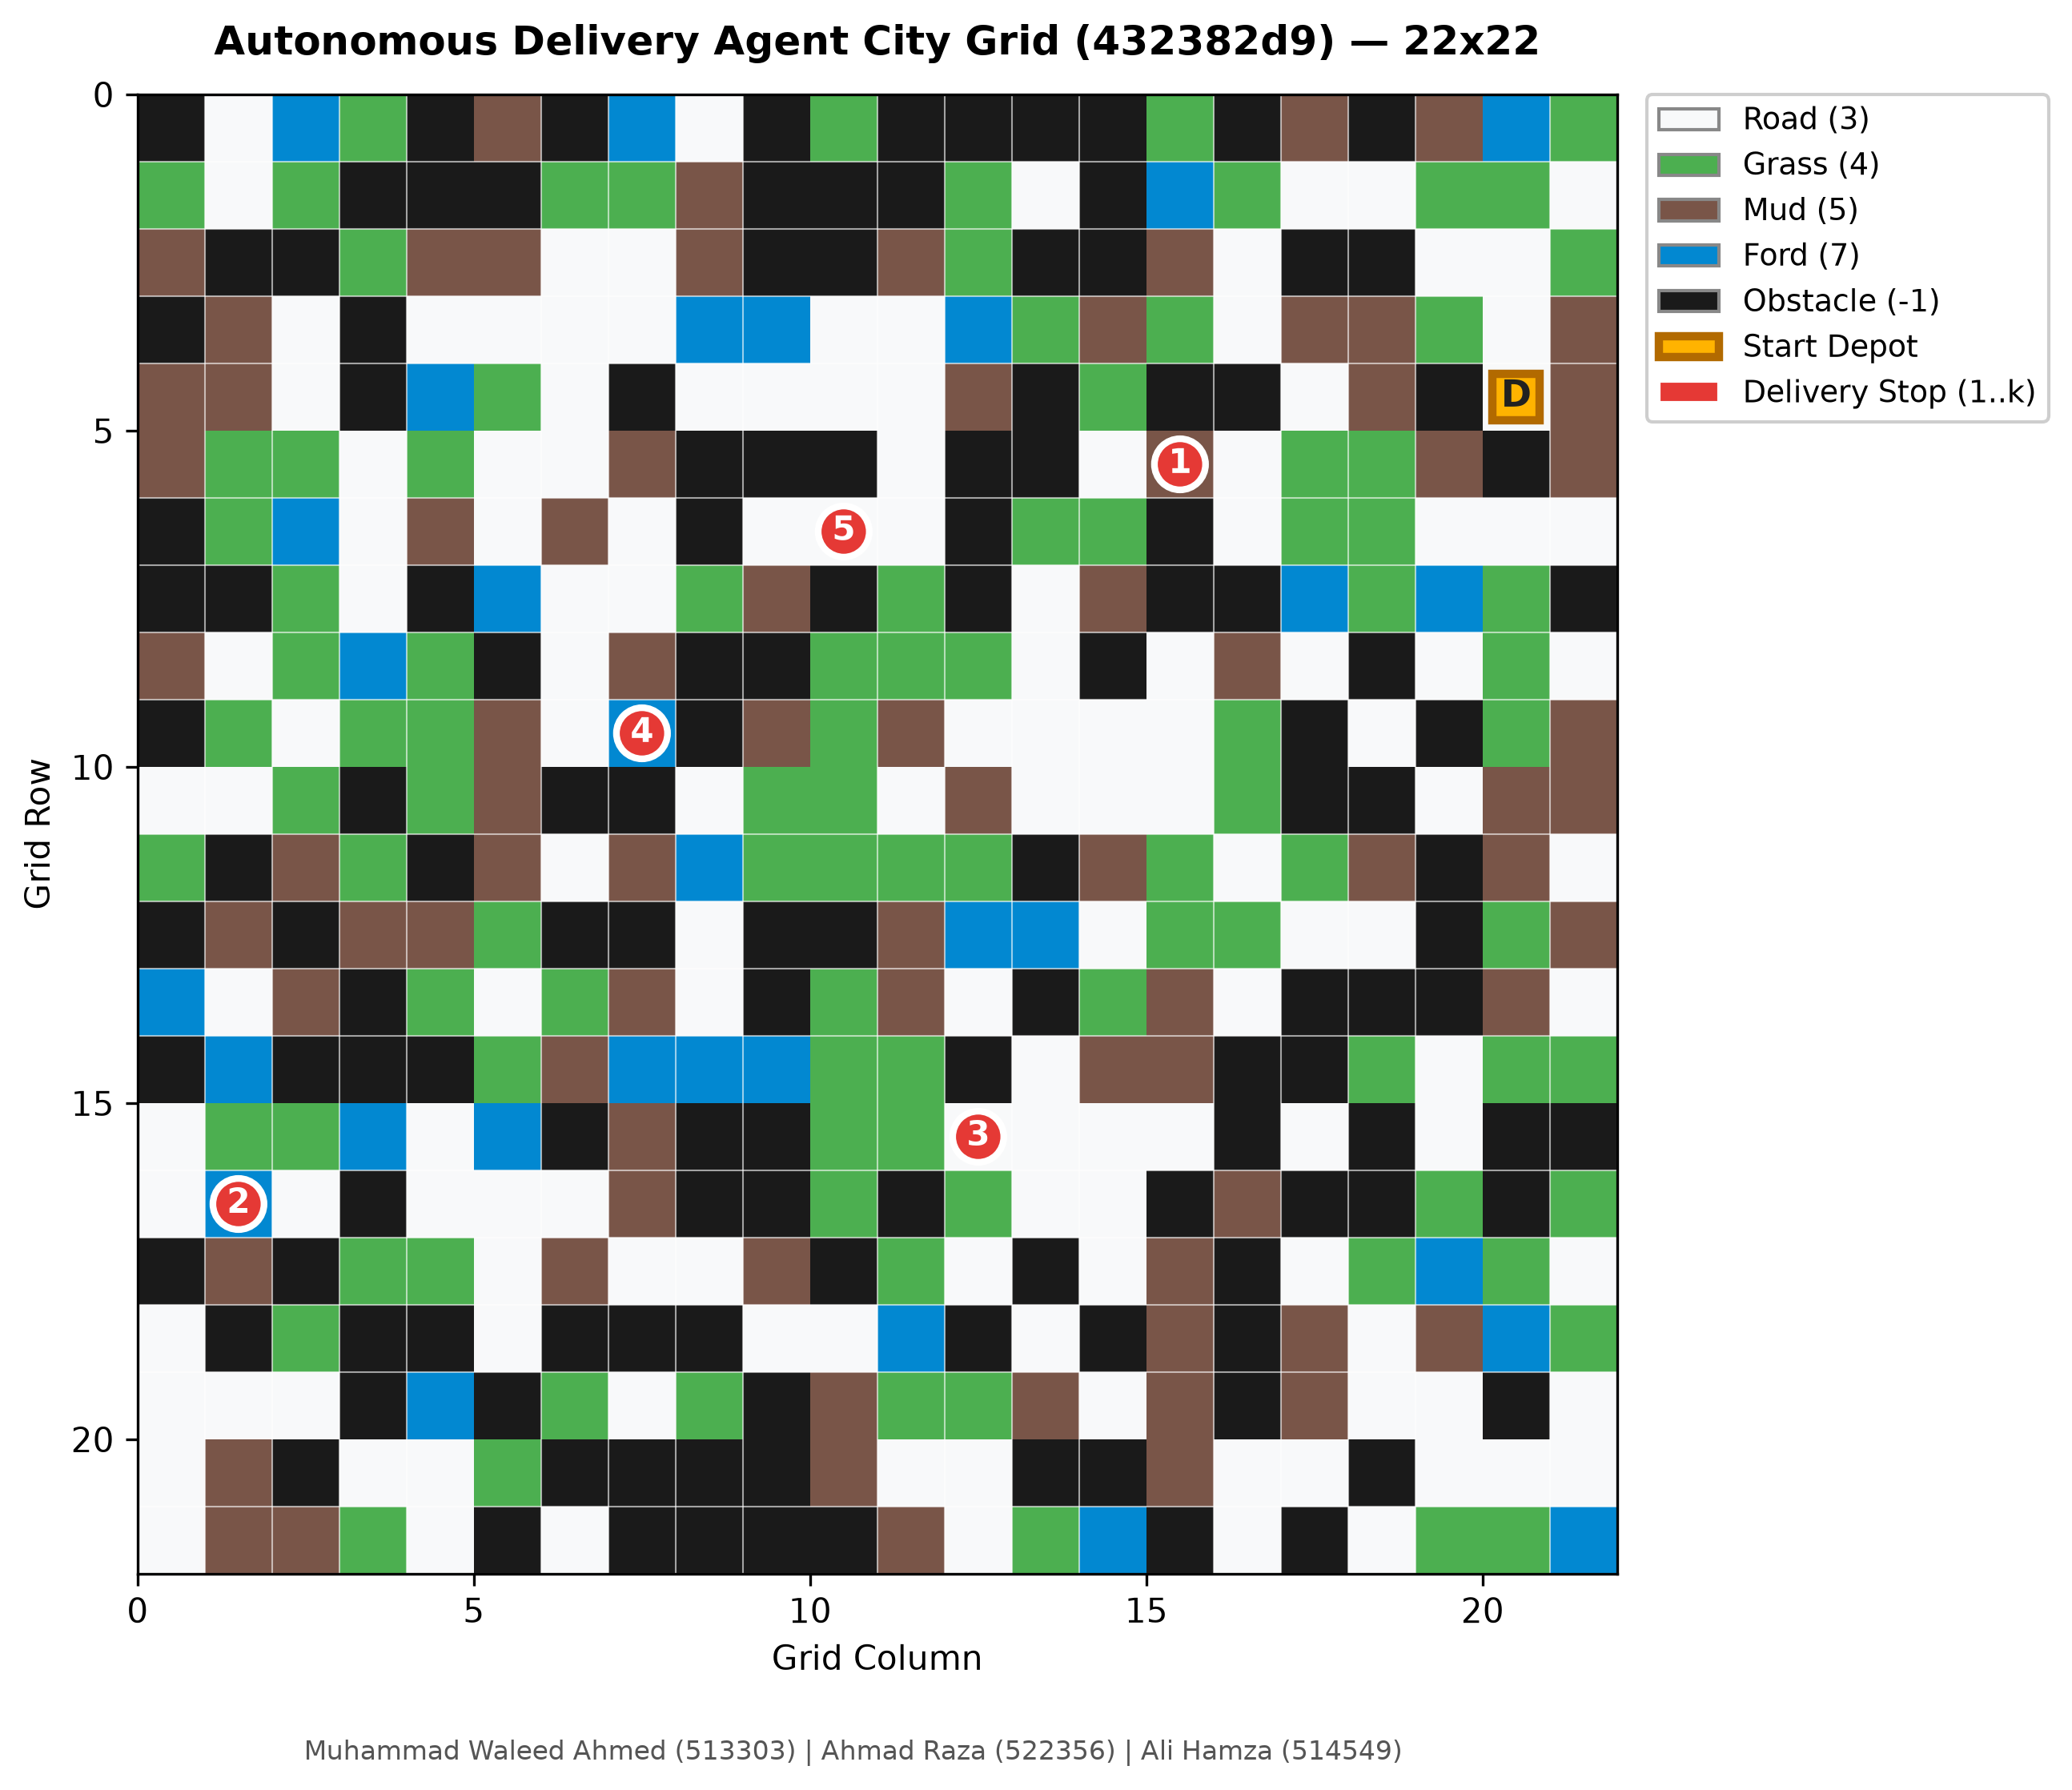
\includegraphics[width=0.90\columnwidth]{canonical_grid.png}
    \caption{Canonical $22 \times 22$ grid instance (\texttt{432382d9}) with depot, 5 stops, and terrain costs. | \stampline}
    \label{fig:canonical_grid}
\end{figure}

\begin{figure}[t]
    \centering
    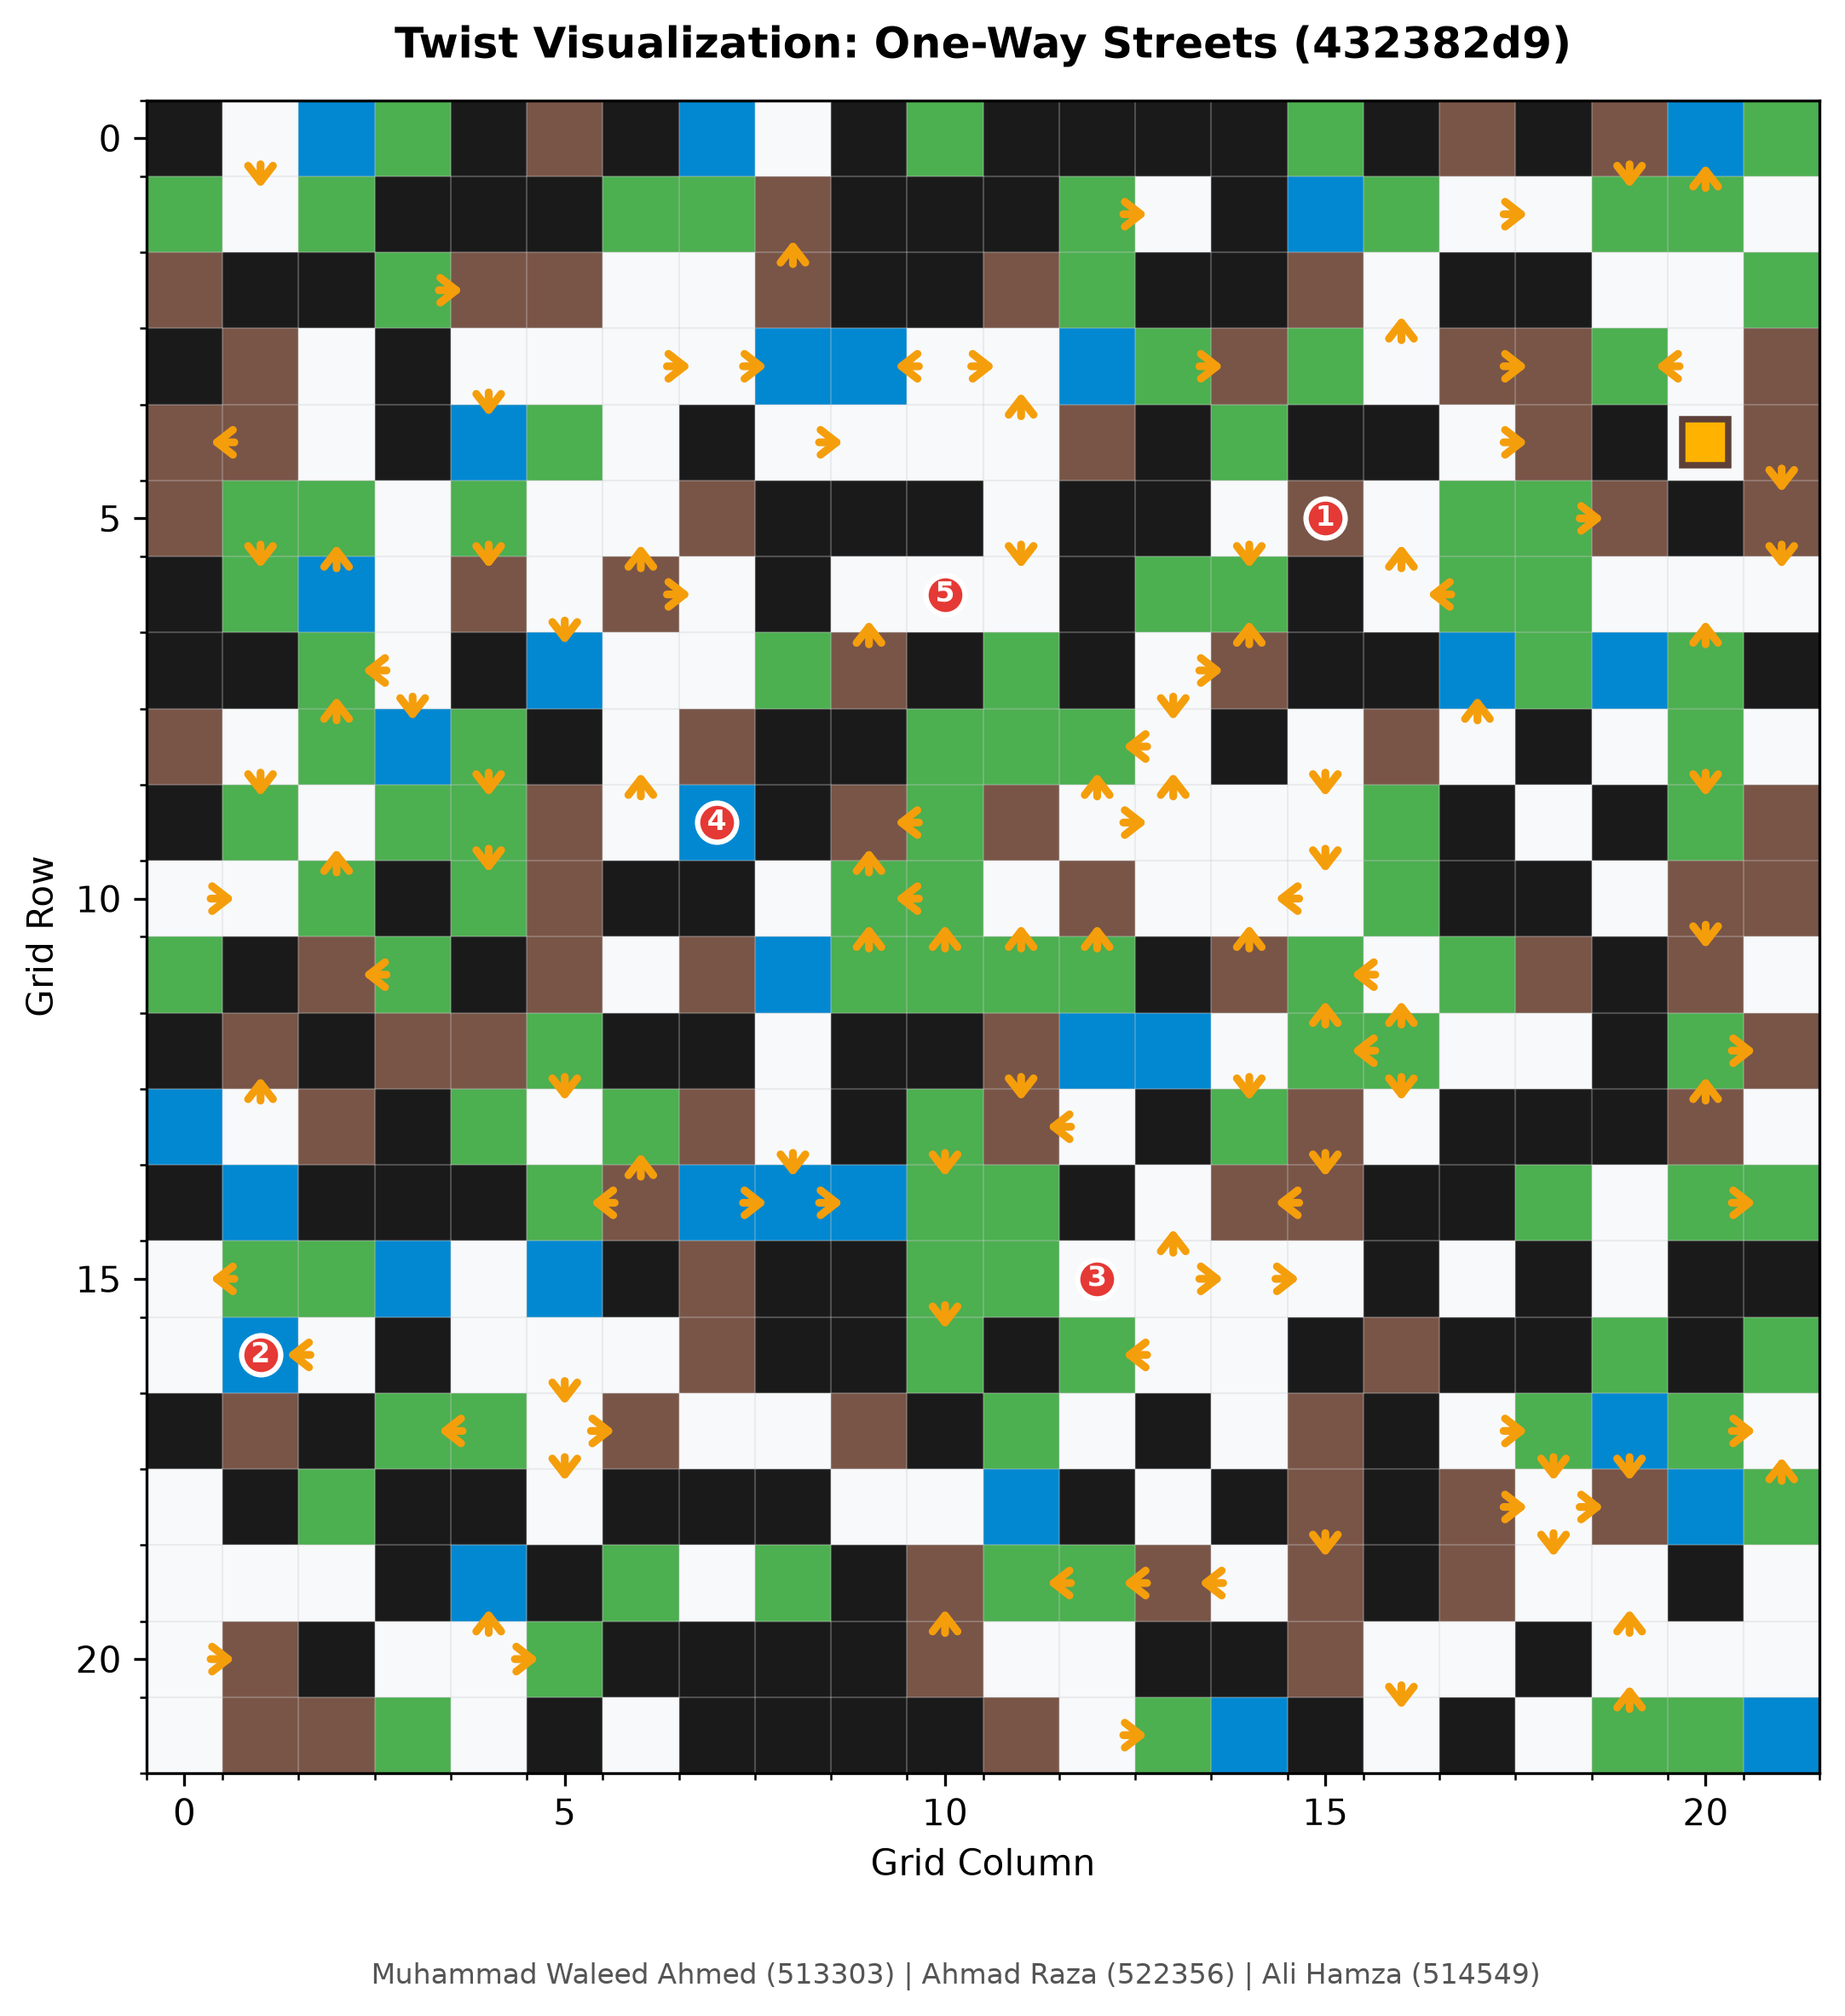
\includegraphics[width=0.90\columnwidth]{twist_one_way.png}
    \caption{Assigned \texttt{one\_way\_streets} directed edge mask on the canonical grid. | \stampline}
    \label{fig:twist_oneway}
\end{figure}

\begin{figure}[t]
    \centering
    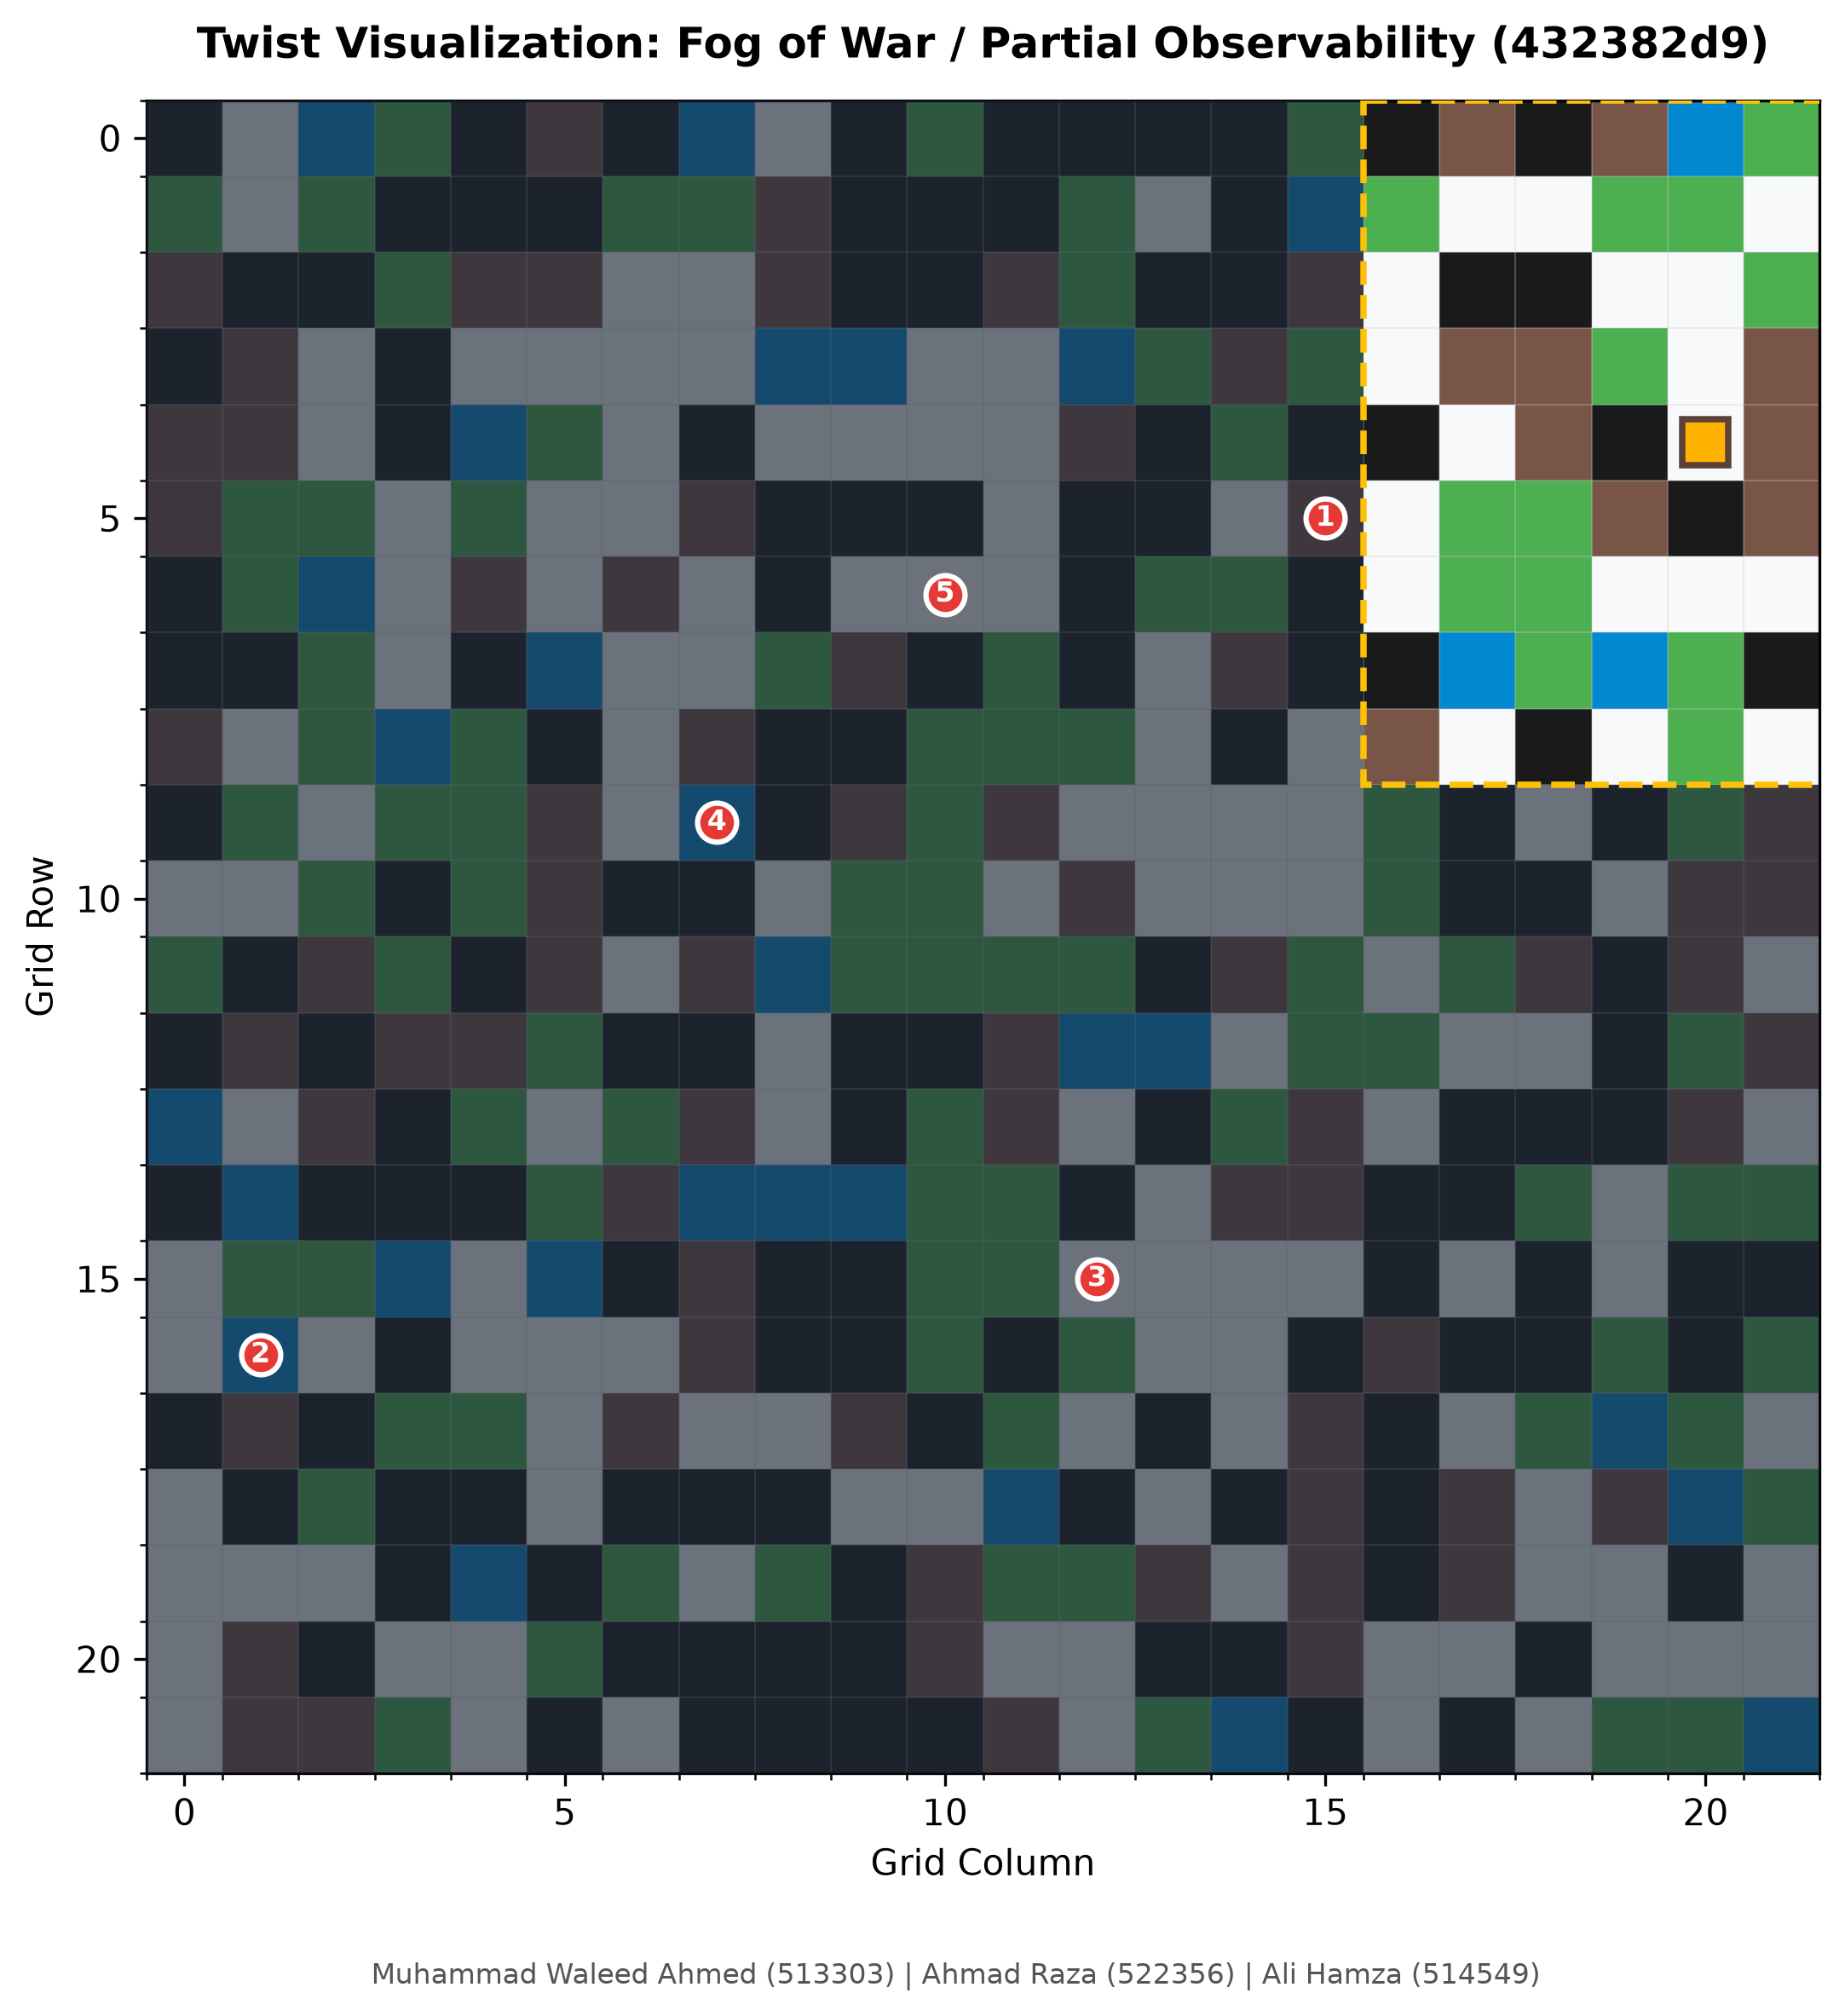
\includegraphics[width=0.90\columnwidth]{twist_fog.png}
    \caption{Assigned \texttt{fog\_partial\_observability} percept radius and belief-map separation. | \stampline}
    \label{fig:twist_fog}
\end{figure}

\begin{figure}[t]
    \centering
    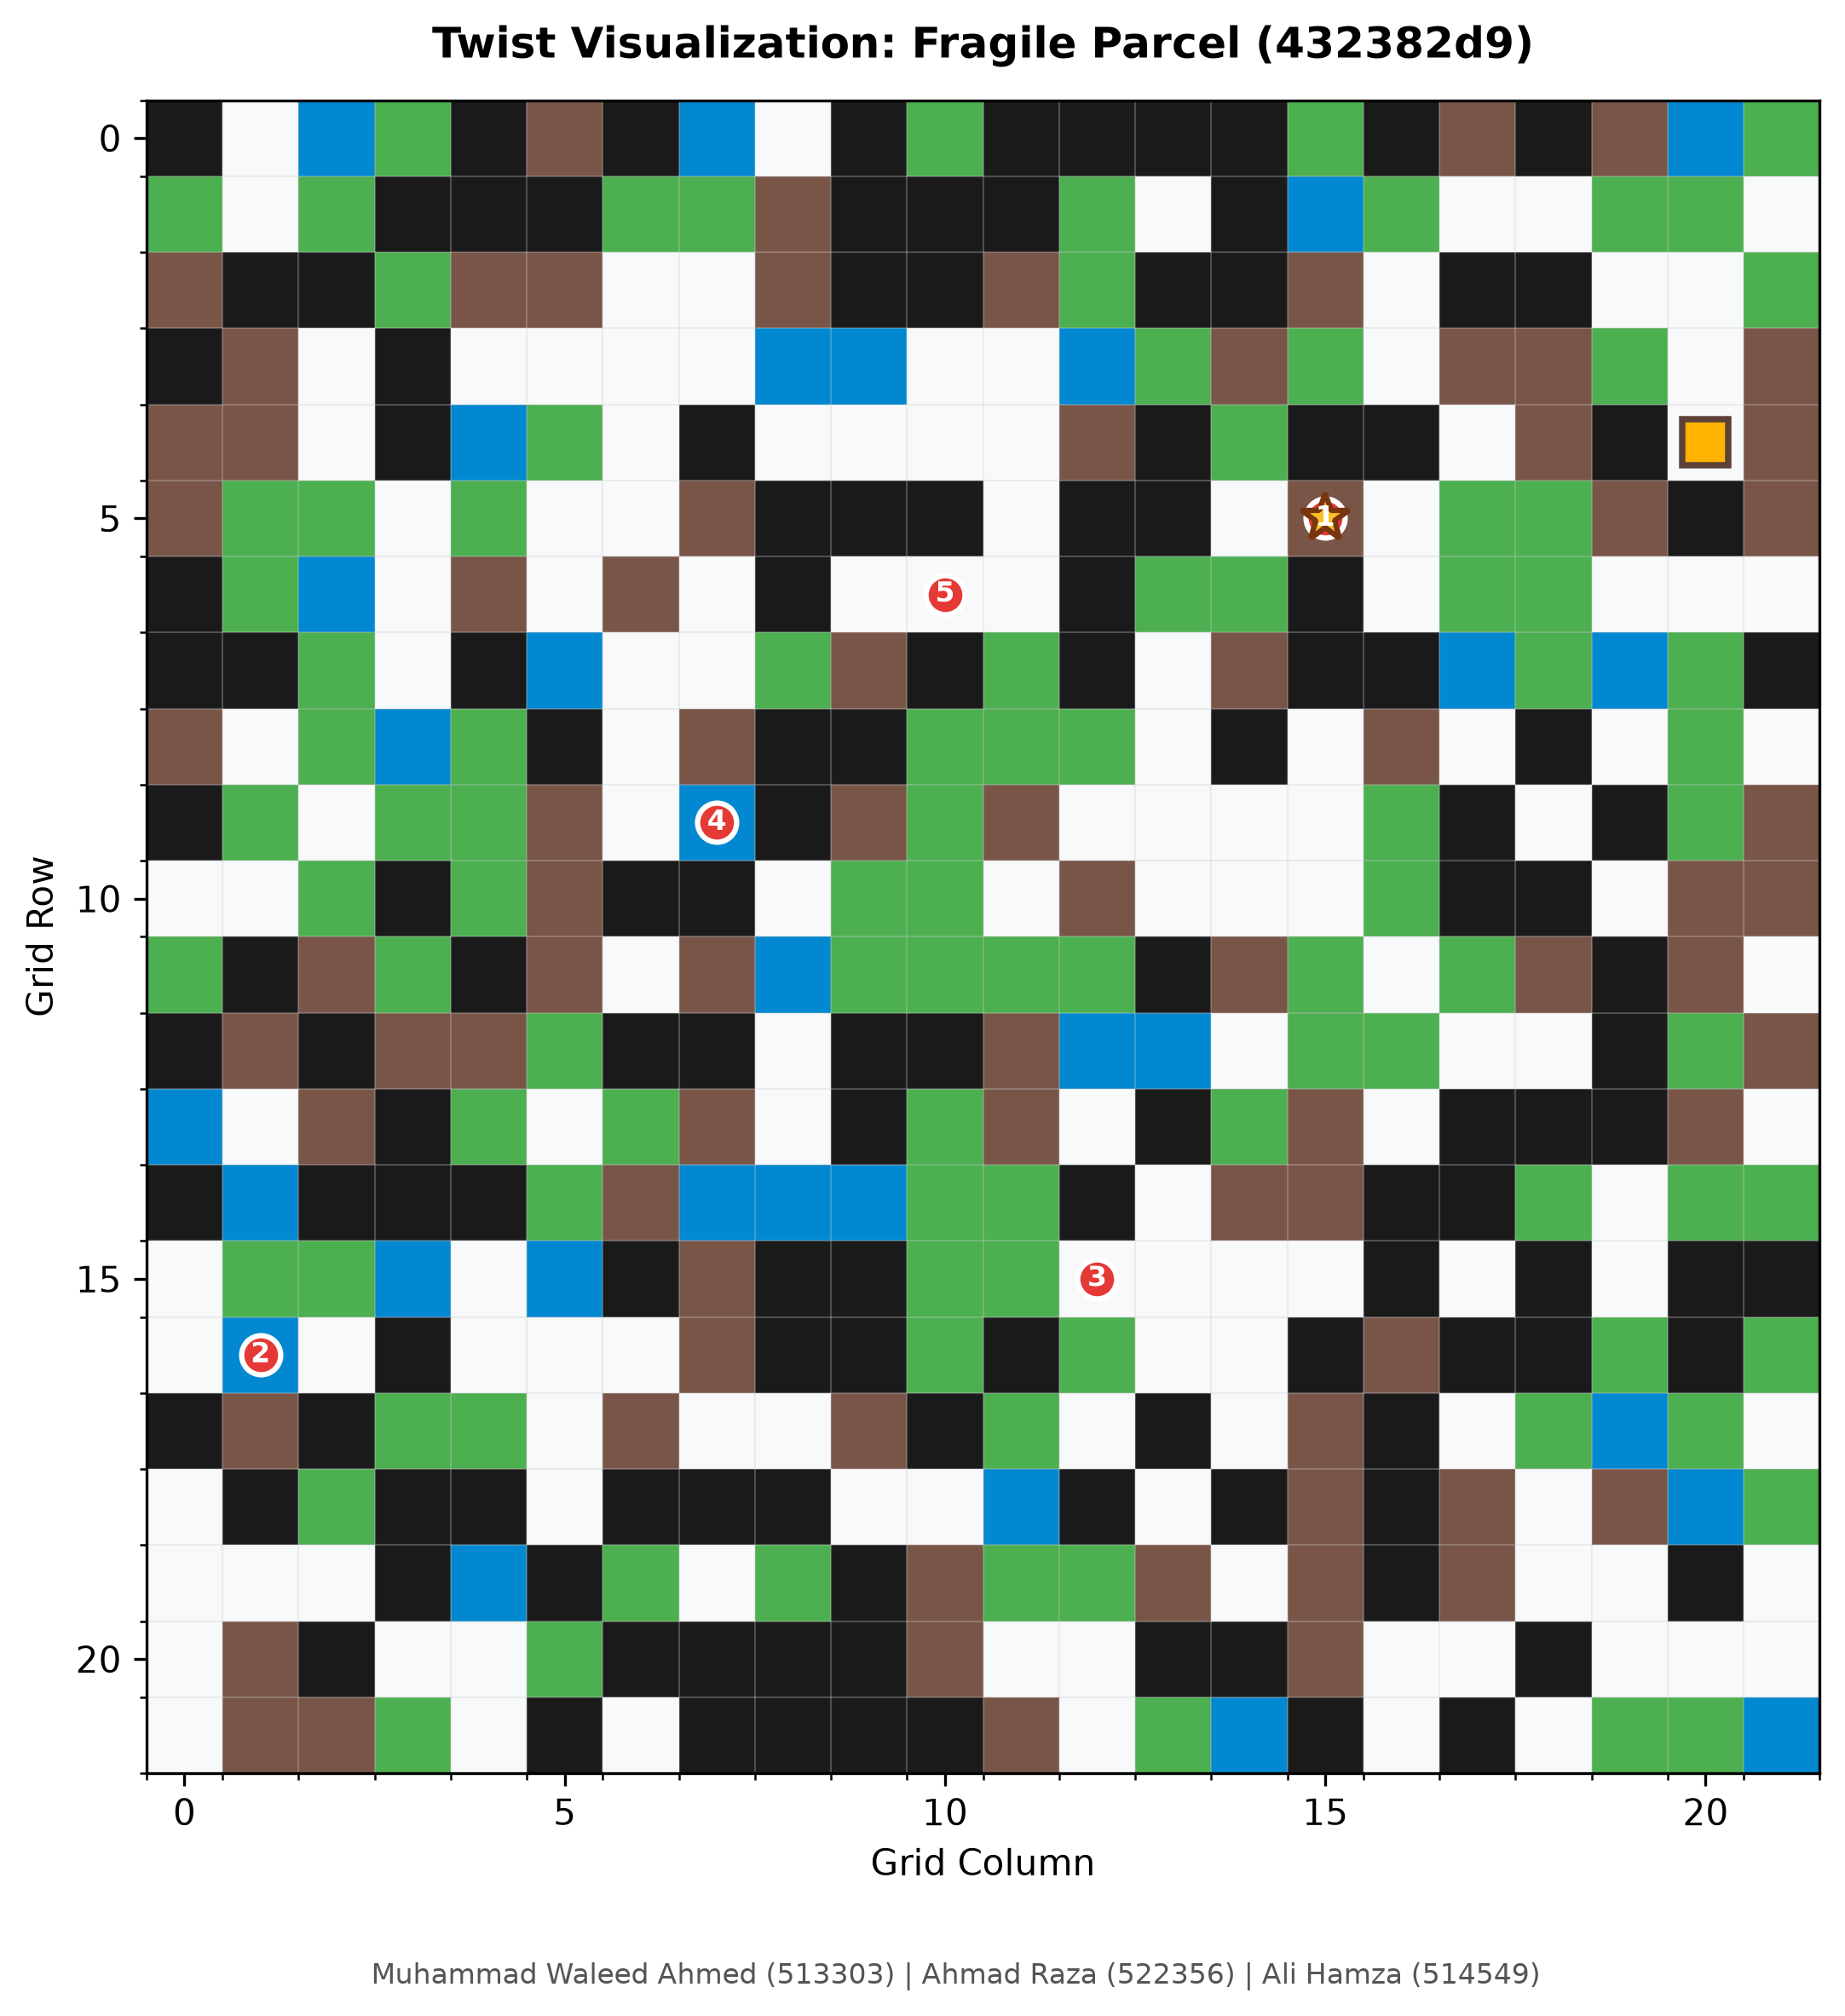
\includegraphics[width=0.90\columnwidth]{twist_fragile.png}
    \caption{Approved third twist \texttt{fragile\_parcel} restricting \texttt{mud}/\texttt{ford} traversal until delivery. | \stampline}
    \label{fig:twist_fragile}
\end{figure}

\section{Part A: World Model and Agent Formalisation}
\subsection{PEAS and Environment Classification}
Tables~\ref{tab:peas} and~\ref{tab:env_class} formalise the PEAS description and six-dimension environment classification incorporating the assigned twists. Under the full problem, the agent operates in a partially observable, stochastic, sequential, semi-dynamic/multi-agent, discrete world.

\begin{table}[t]
    \centering
    \caption{PEAS Formulation Including Assigned Twists. | \stampline}
    \label{tab:peas}
    \scriptsize
    \begin{tabular}{@{}p{1.6cm}p{6.5cm}@{}}
        \toprule
        \textbf{Component} & \textbf{Specification} \\
        \midrule
        Performance & Deliver all 5 parcels, minimise total terrain cost, avoid capture/theft ($C \le \kappa C^*$). \\
        Environment & $22\times 22$ grid, terrain $\{3,4,5,7\}$, walls ($-1$), one-way edges, fog radius $\rho$, \texttt{chaser} rival. \\
        Actuators & Cardinal moves $\{N, E, S, W\}$ (subject to slip $p=0.23$) and \texttt{WAIT} in game mode. \\
        Sensors & Agent/rival coordinates, delivered bitmask, local percept grid within radius $\rho$. \\
        \bottomrule
    \end{tabular}
\end{table}

\begin{table}[t]
    \centering
    \caption{Environment Classification Across Six Standard Dimensions. | \stampline}
    \label{tab:env_class}
    \scriptsize
    \begin{tabular}{@{}p{2.1cm}p{2.0cm}p{3.8cm}@{}}
        \toprule
        \textbf{Dimension} & \textbf{Classification} & \textbf{Twist / World Justification} \\
        \midrule
        Observability & Partially Observable & Fog radius $\rho$ hides distant cells. \\
        Determinism & Stochastic & Simulator slip ($p=0.23$) deflects moves. \\
        Episodic/Seq. & Sequential & Parcel mask and fragile/one-way rules couple steps. \\
        Static/Dynamic & Semi-Dynamic & Static terrain; rival moves on alternating plies. \\
        Discrete/Cont. & Discrete & Finite grid cells, discrete actions, integer costs. \\
        Single/Multi & Multi-Agent & Single-agent in Part B; \texttt{chaser} rival in Part C. \\
        \bottomrule
    \end{tabular}
\end{table}

\subsection{Agent Type and Simple Reflex Failure}
Our courier is a \textbf{utility-based agent}: it minimises cumulative terrain entry cost in Part B and trades off route progress against rival capture risk in Part C. A simple reflex agent fails because it lacks memory of visited cells and delivered stops, becoming trapped in wall concavities and local cost minima (Fig.~\ref{fig:reflex_fail}). Across \numPartaReflexScenarios{} certified scenarios, the simple reflex baseline succeeded in only \numPartaReflexSuccesses/\numPartaReflexScenarios{} (\numPartaReflexSuccessPct{}\%, 95\% Wilson CI $[0.6\%, 16.7\%]$).

\begin{figure}[t]
    \centering
    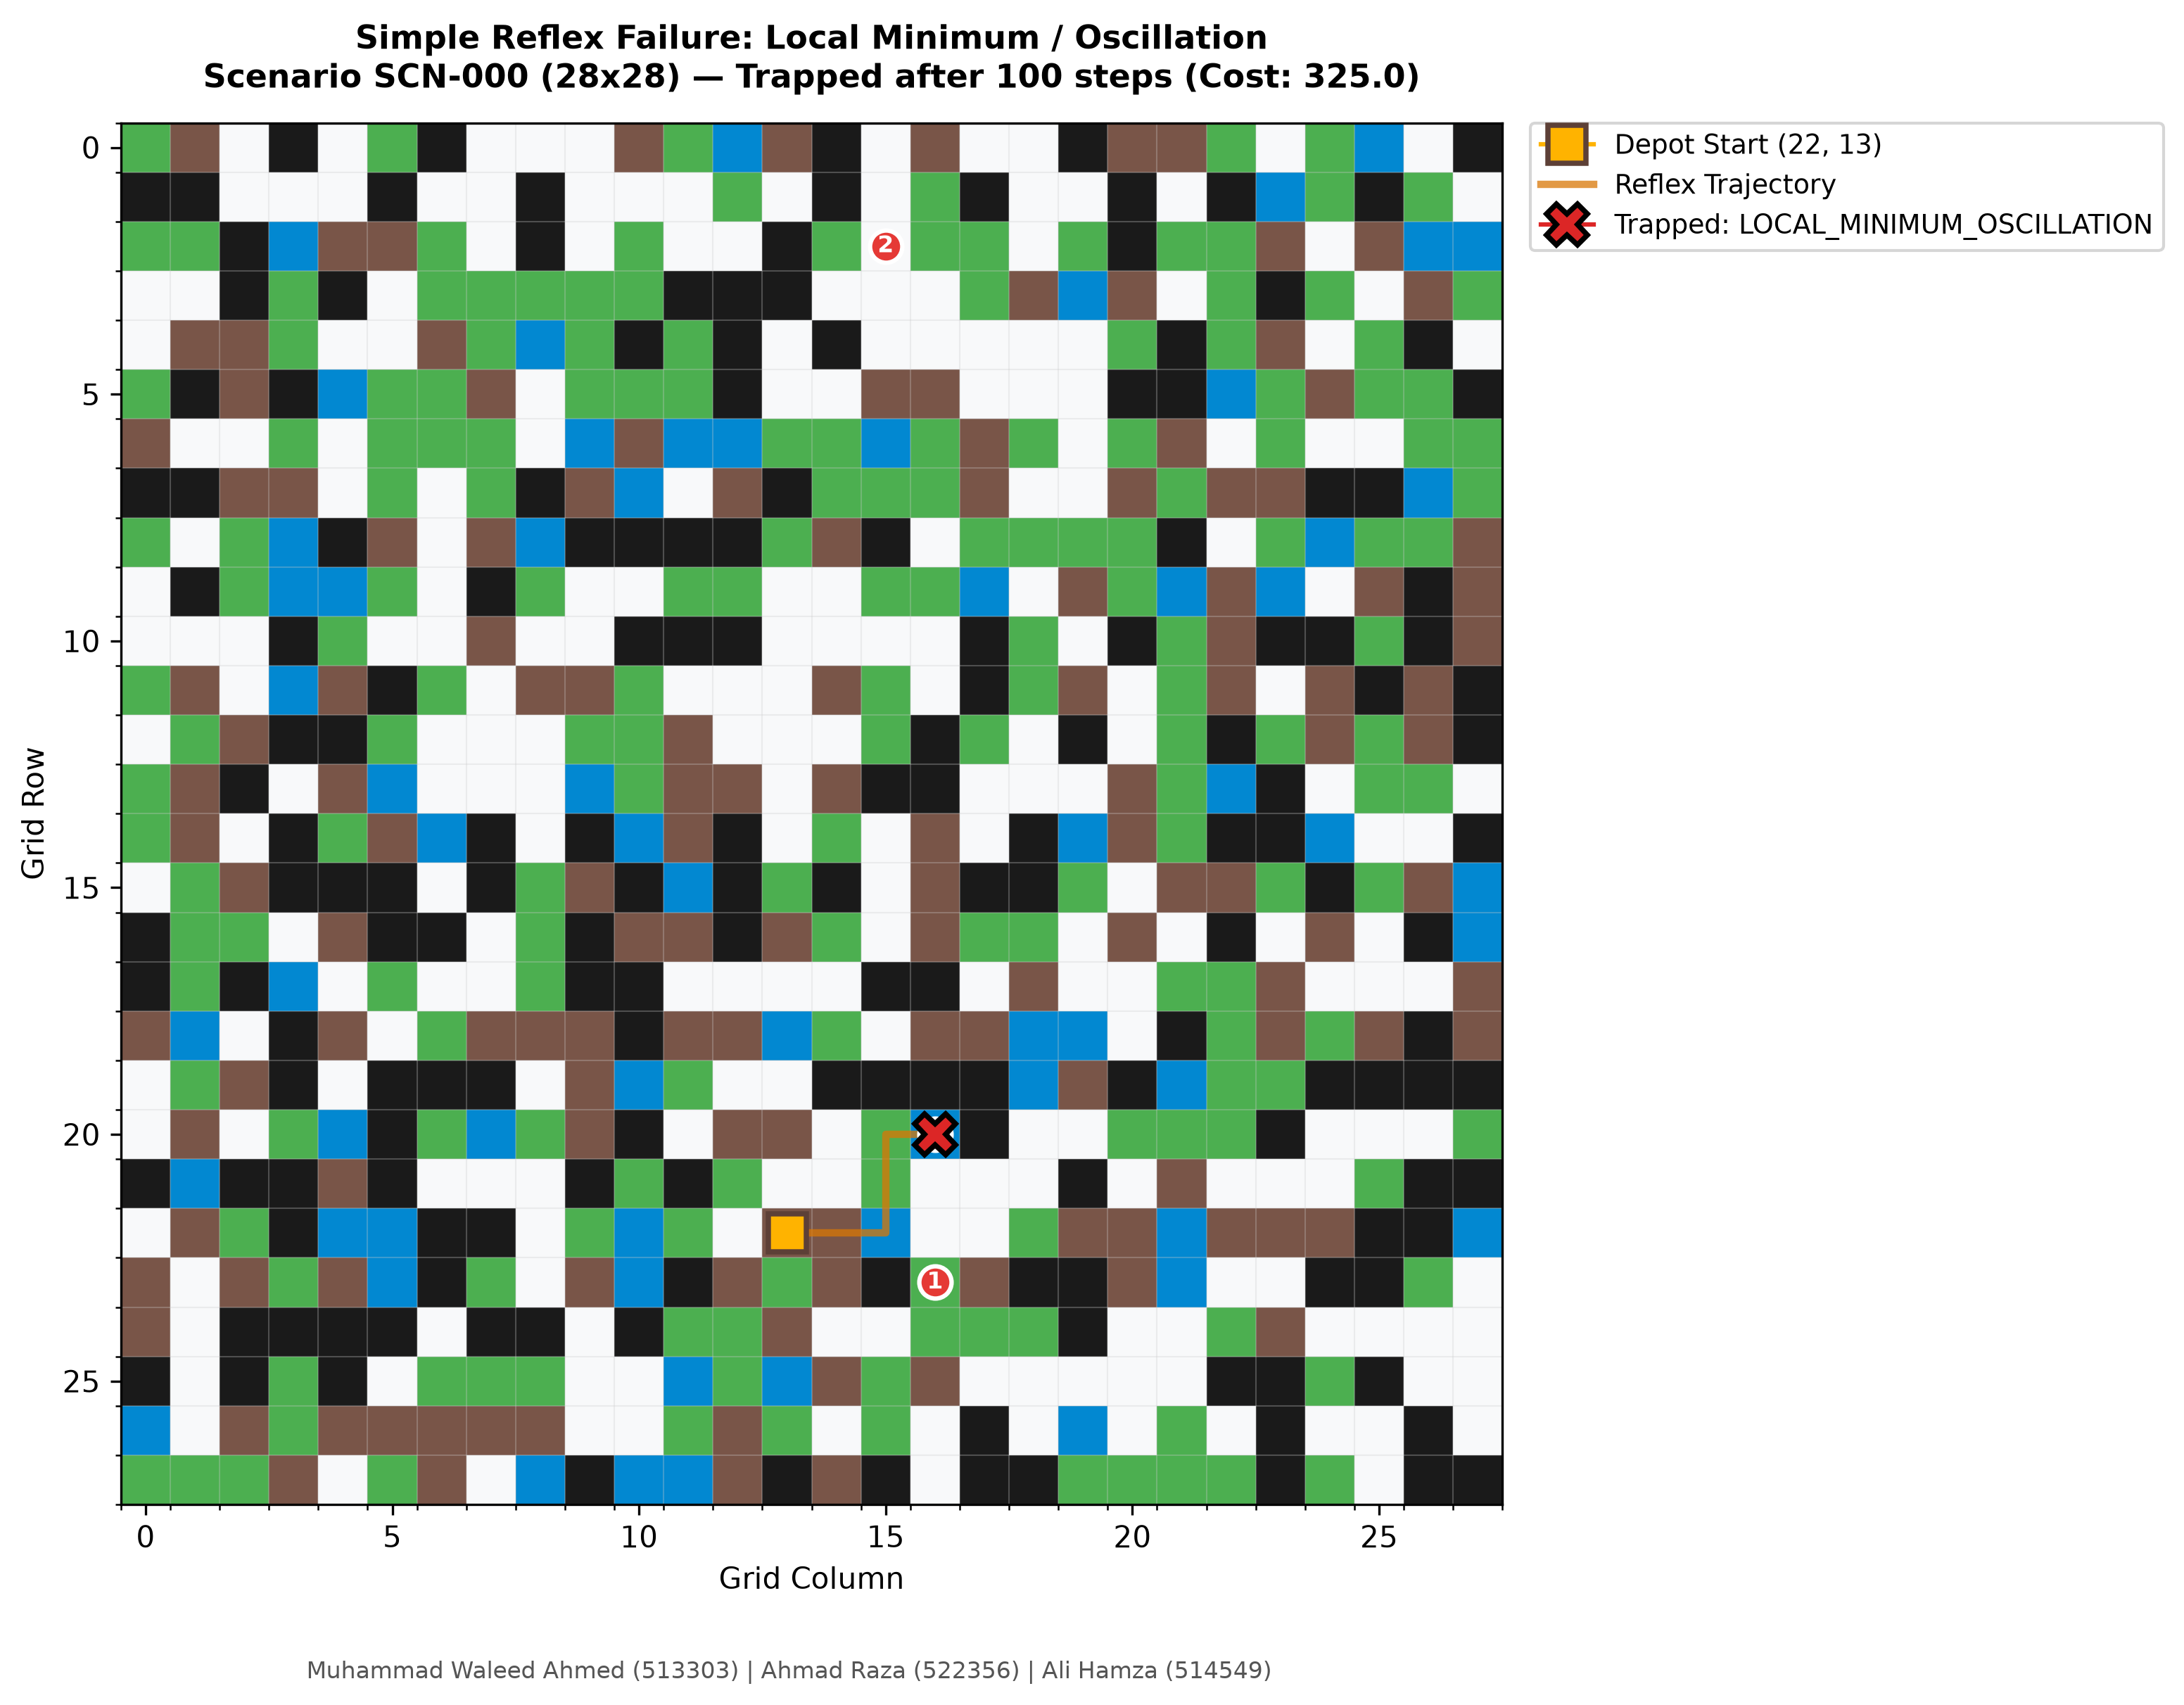
\includegraphics[width=0.90\columnwidth]{partA_reflex_failure.png}
    \caption{Simple reflex agent oscillating in a wall concavity without search memory. | \stampline}
    \label{fig:reflex_fail}
\end{figure}

\subsection{NumPy Vectorisation Benchmark}
We implemented cost-map construction and neighbour-legality checks using vectorised NumPy array slicing and compared against a pure-Python nested-loop reference across grid sizes $N \in \{20, 22, 30, 200, 1000\}$ (Table~\ref{tab:speedup}, Fig.~\ref{fig:speedup}). Vectorisation eliminates interpreter loop overhead, achieving a $9.95\times$ speedup at $N=1000$ ($10^6$ cells: $3701.0$\,ms loop vs.\ $372.1$\,ms vectorised).

\begin{table}[t]
    \centering
    \caption{Pure-Python Loop vs.\ NumPy Vectorised Cost-Map Runtime. | \stampline}
    \label{tab:speedup}
    \scriptsize
    \begin{tabular}{@{}rrrrr@{}}
        \toprule
        $N$ & Cells & Loop Mean (ms) & Vec Mean (ms) & Speedup \\
        \midrule
        20   & 400       & 1.626    & 0.308   & $5.28\times$ \\
        22   & 484       & 0.708    & 0.308   & $2.30\times$ \\
        30   & 900       & 1.214    & 0.381   & $3.18\times$ \\
        200  & 40,000    & 88.341   & 11.592  & $7.62\times$ \\
        1000 & 1,000,000 & 3701.035 & 372.060 & $9.95\times$ \\
        \bottomrule
    \end{tabular}
\end{table}

\begin{figure}[t]
    \centering
    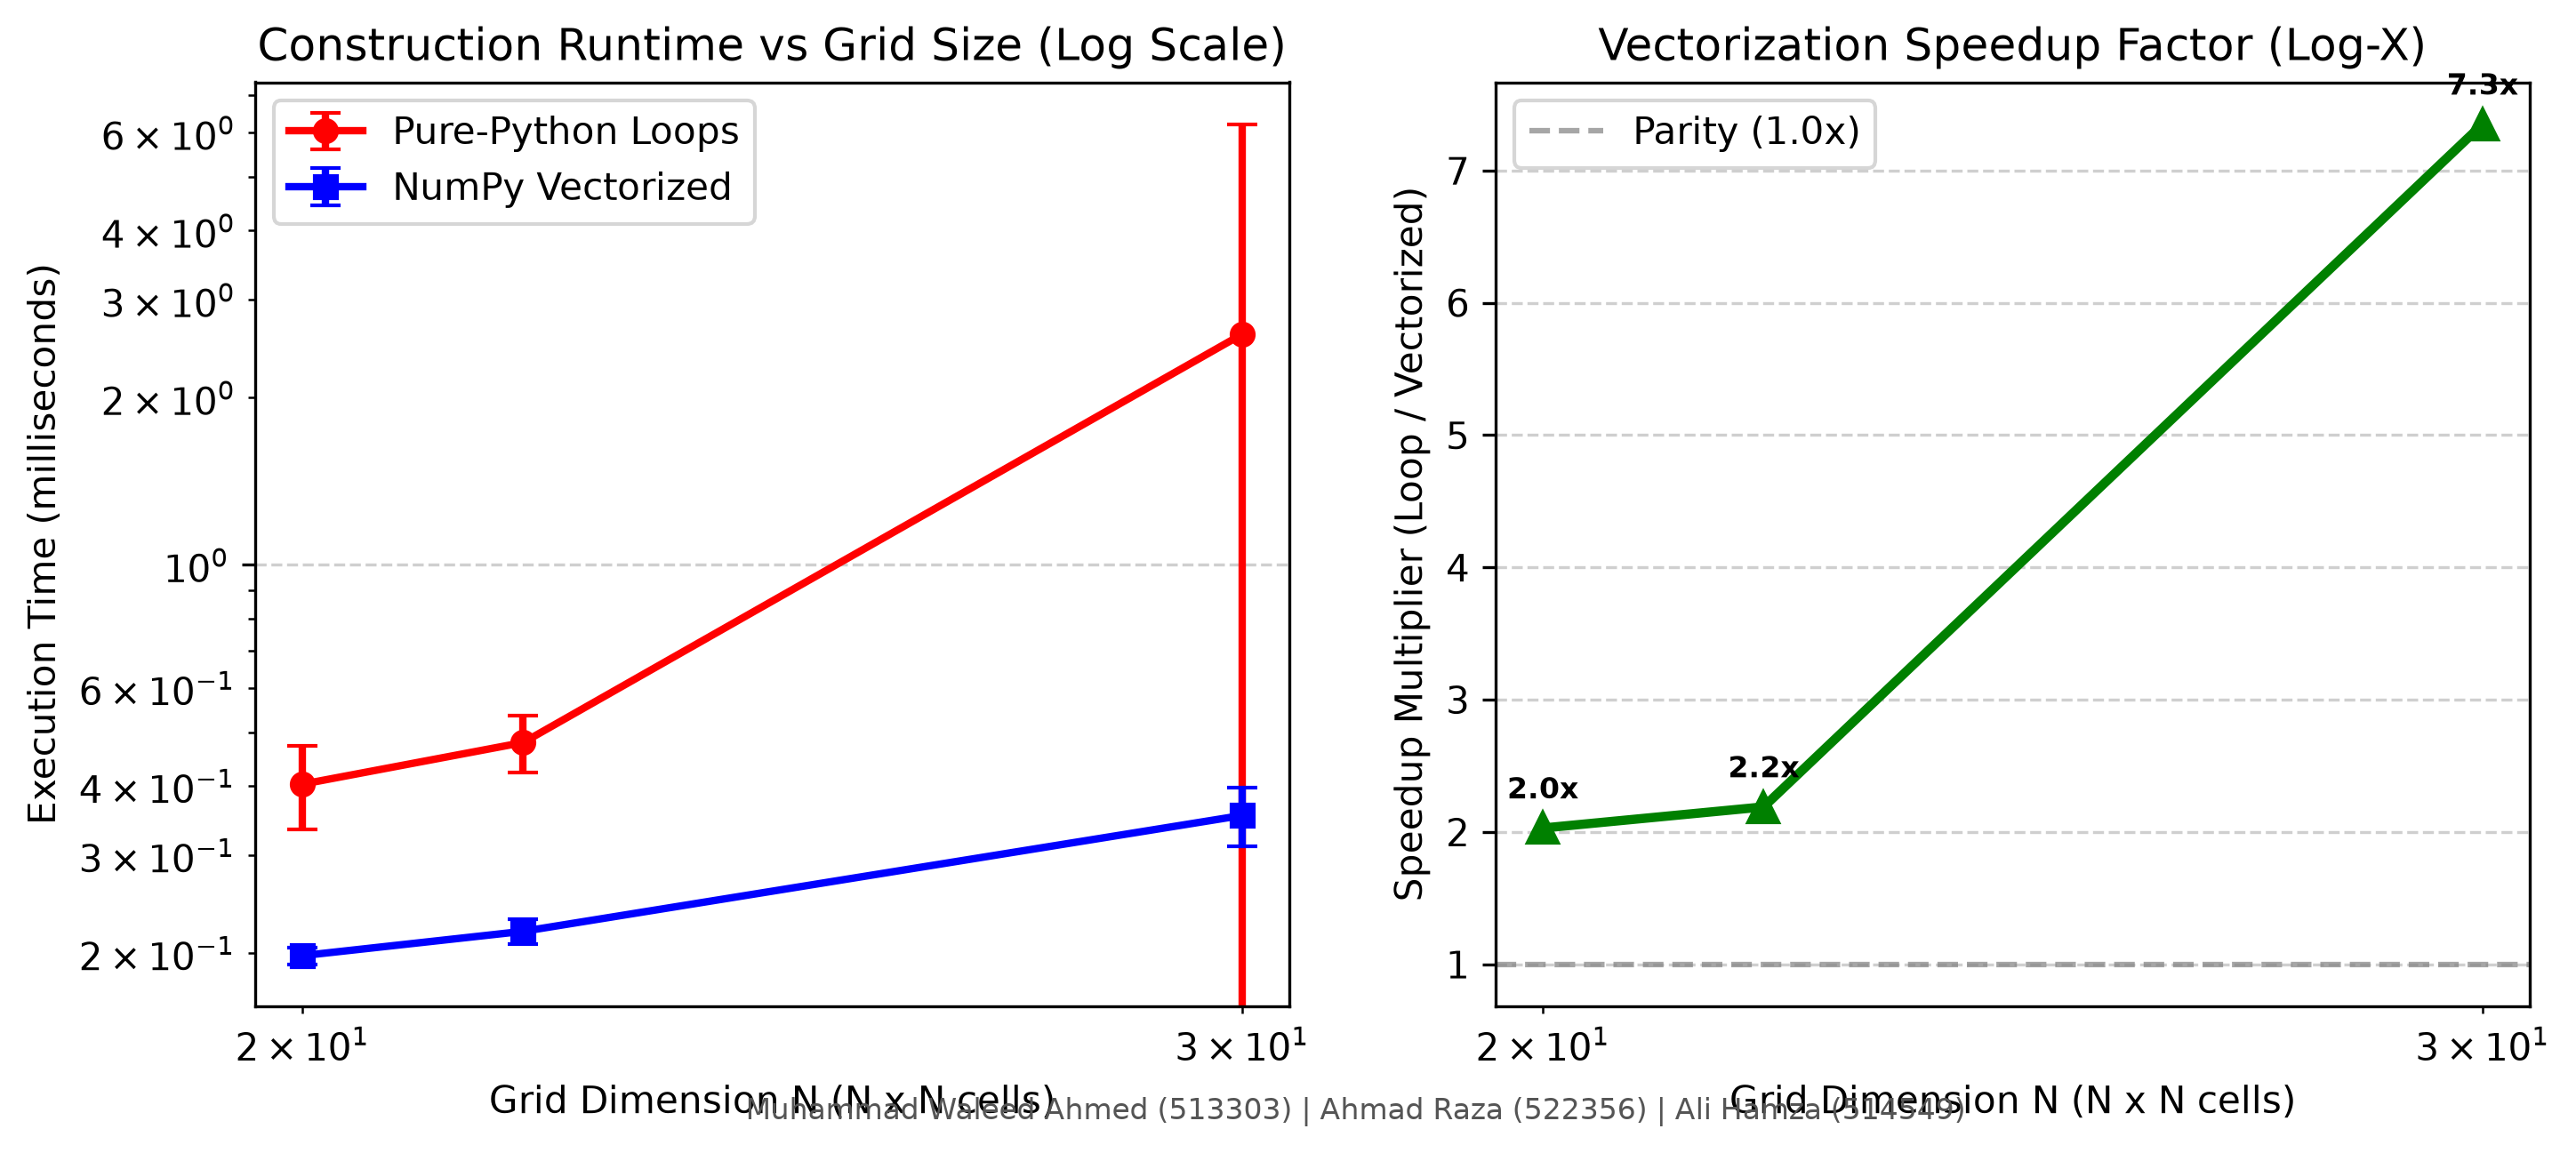
\includegraphics[width=0.90\columnwidth]{partA_speedup.png}
    \caption{Vectorised NumPy vs.\ pure-Python loop runtime scaling across $N=20..1000$. | \stampline}
    \label{fig:speedup}
\end{figure}

\section{Part B: Multi-Stop Route Planning}
\subsection{Search Formulation and Algorithms}
We formulate multi-stop delivery as a single deterministic search problem with hashable state $s = (p, \text{mask}, \text{extra})$, where $p = r \cdot n + c$ is the flat cell index, $\text{mask} \in [0, 2^K - 1]$ is the delivered-stop bitmask, and $\text{extra}$ holds twist-specific state variables. Entering a stop cell automatically sets its bit in $\text{mask}$. All edge costs are finite and strictly positive ($c(s,a,s') > 0$). We implemented BFS, UCS, DLS, IDS, Greedy Best-First, and A* from scratch \cite{russell2020aima,hart1968astar,korf1985ida}, with deterministic action ordering $(N, E, S, W)$.

\subsection{Custom Heuristic and Admissibility Proof}
To solve multi-stop routing efficiently under \texttt{one\_way\_streets} and obstacles, we designed \texttt{CombinedMSTHeuristic}:
\begin{equation}
    h_{\text{own}}(s) = \max\bigl(h_{\text{MST}}(s),\, h_{B2}(s)\bigr),
\end{equation}
where $h_{B2}(s) = \max_{i \in U} d_{\text{dir}}(p, u_i)$ is the maximum reverse-Dijkstra directed distance from position $p$ to any undelivered stop $u_i \in U$ on the relaxed graph (ignoring fragile/resource restrictions while respecting walls and one-way edges). For $h_{\text{MST}}(s)$, we construct a Minimum Spanning Tree over $\{p\} \cup U$ using symmetric lower-bound edge weights $w(u,v) = \min\bigl(d_{\text{dir}}(u,v), d_{\text{dir}}(v,u)\bigr)$.

\textbf{Admissibility Proof:} Any valid remaining tour $\pi^*$ from $p$ visiting all $u \in U$ induces a connected spanning subgraph on $\{p\} \cup U$ whose directed path costs satisfy $c_{\text{dir}}(u,v) \ge d_{\text{dir}}(u,v) \ge w(u,v)$. Deleting one edge from a spanning tour yields a spanning tree of weight at most $\text{cost}(\pi^*)$; since Prim's algorithm finds the minimum-weight spanning tree, $h_{\text{MST}}(s) \le h^*(s)$. Likewise, $h_{B2}(s) \le h^*(s)$ because every stop $u_i \in U$ must be reached. Since both terms lower-bound $h^*(s)$, their maximum $h_{\text{own}}(s)$ is admissible. Empirical consistency checks across sampled transitions confirmed zero monotonicity violations.

\subsection{Empirical Search Comparison}
Table~\ref{tab:six_algos} and Fig.~\ref{fig:six_algos} report the six-algorithm benchmark across \numPartbScenarios{} certified scenarios (limits: $2\times 10^6$ expansions, $60$\,s). BFS minimises move count ($71.9$ moves, suboptimal cost $253.73$), whereas UCS and A* find cost-optimal routes (\numPartbOwnMeanCost{}). DLS ($d=10$, $d=25$) and IDS fail on 5-stop instances due to depth cutoff or node/time limits. Compared against baselines (Table~\ref{tab:heuristics}, Fig.~\ref{fig:heuristics}), A* with $h_{\text{own}}$ expands \numPartbOwnMeanExp{} nodes versus \numPartbBTwoMeanExp{} for B2 (Max Relaxed), $9235.2$ for B1 (Manhattan), and \numPartbUcsMeanExp{} for UCS. Fig.~\ref{fig:plan_own} illustrates the resulting optimal A* route on the canonical grid.

\begin{table}[t]
    \centering
    \caption{Six-Algorithm Comparison Across \numPartbScenarios{} Certified Scenarios. | \stampline}
    \label{tab:six_algos}
    \scriptsize
    \begin{tabular}{@{}lrrrr@{}}
        \toprule
        Algorithm & Solved & Expansions (Mean) & Cost & Peak Stored \\
        \midrule
        BFS                 & 30/30 & 11977.6 & 253.73 & 12665.6 \\
        UCS                 & 30/30 & \numPartbUcsMeanExp{} & \numPartbOwnMeanCost{} & 13140.0 \\
        DLS ($d=10$)        & 0/30  & CUTOFF  & DNF    & 20.0 \\
        DLS ($d=25$)        & 0/30  & NODELIMIT & DNF  & 50.0 \\
        IDS                 & 0/30  & NODELIMIT/TIMEOUT & DNF & 34.1 \\
        Greedy ($h_{\text{own}}$) & 30/30 & 133.7 & 273.27 & 272.5 \\
        A* ($h_{\text{own}}$)     & 30/30 & \numPartbOwnMeanExp{} & \numPartbOwnMeanCost{} & 658.5 \\
        \bottomrule
    \end{tabular}
\end{table}

\begin{table}[t]
    \centering
    \caption{Heuristic Comparison on A* Across \numPartbScenarios{} Scenarios. | \stampline}
    \label{tab:heuristics}
    \scriptsize
    \begin{tabular}{@{}lrrrr@{}}
        \toprule
        Heuristic & Solved & Expansions (95\% CI) & Time (s) & Cost \\
        \midrule
        UCS ($h=0$)      & 30/30 & \numPartbUcsMeanExp{} [7228.2, 17371.0] & 0.579 & \numPartbOwnMeanCost{} \\
        B1 (Manhattan)   & 30/30 & 9235.2 [4952.7, 13517.8]  & 0.481 & 218.43 \\
        B2 (Max Directed)& 30/30 & \numPartbBTwoMeanExp{} [1505.5, 5194.3]   & 0.224 & \numPartbOwnMeanCost{} \\
        Own (Combined)   & 30/30 & \numPartbOwnMeanExp{} [246.3, 528.6]      & 0.059 & \numPartbOwnMeanCost{} \\
        \bottomrule
    \end{tabular}
\end{table}

\begin{figure}[t]
    \centering
    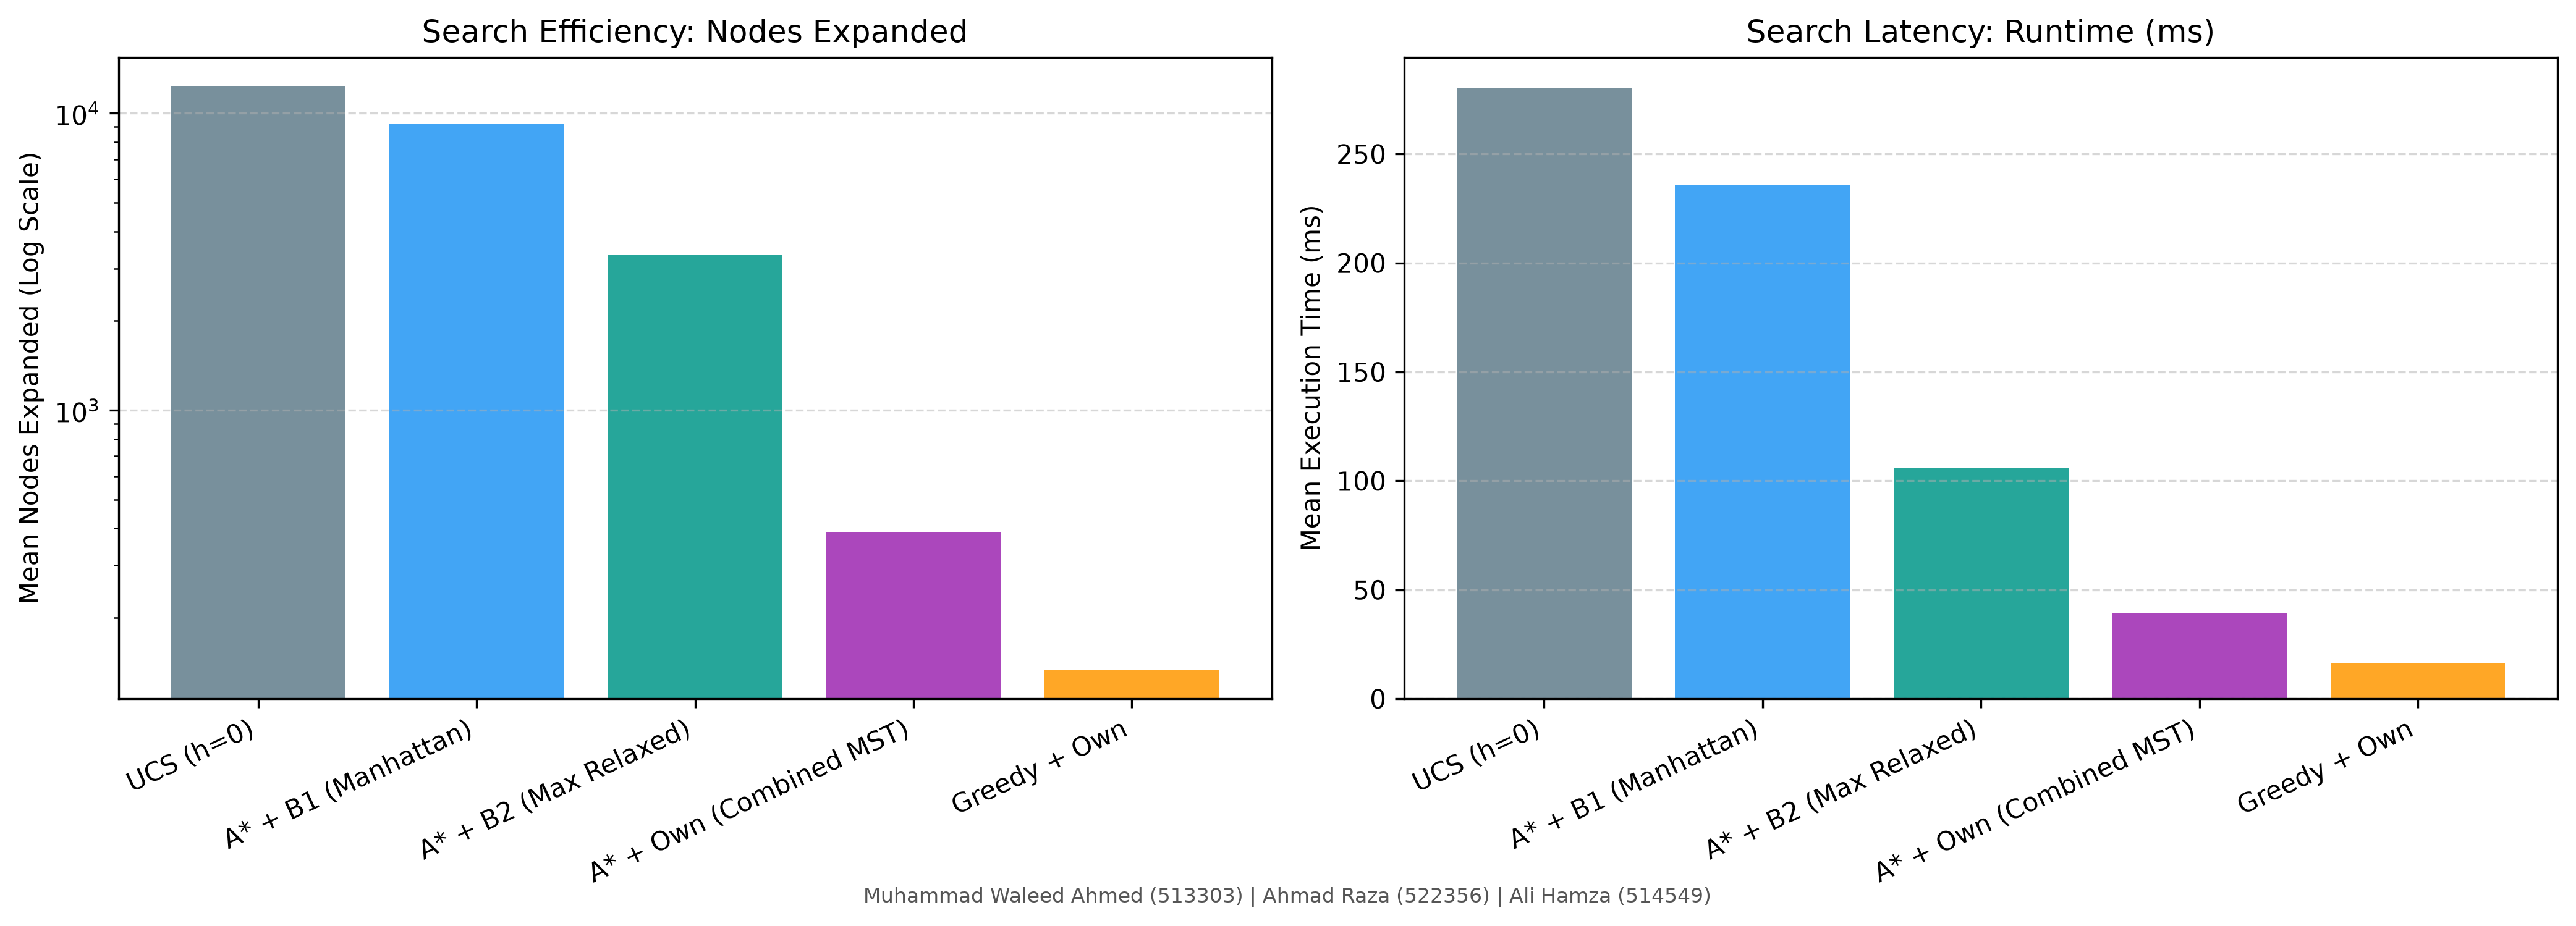
\includegraphics[width=0.90\columnwidth]{partB_heuristics_comparison.png}
    \caption{Node expansions and runtime across UCS, B1, B2, and \texttt{CombinedMSTHeuristic}. | \stampline}
    \label{fig:heuristics}
\end{figure}

\begin{figure}[t]
    \centering
    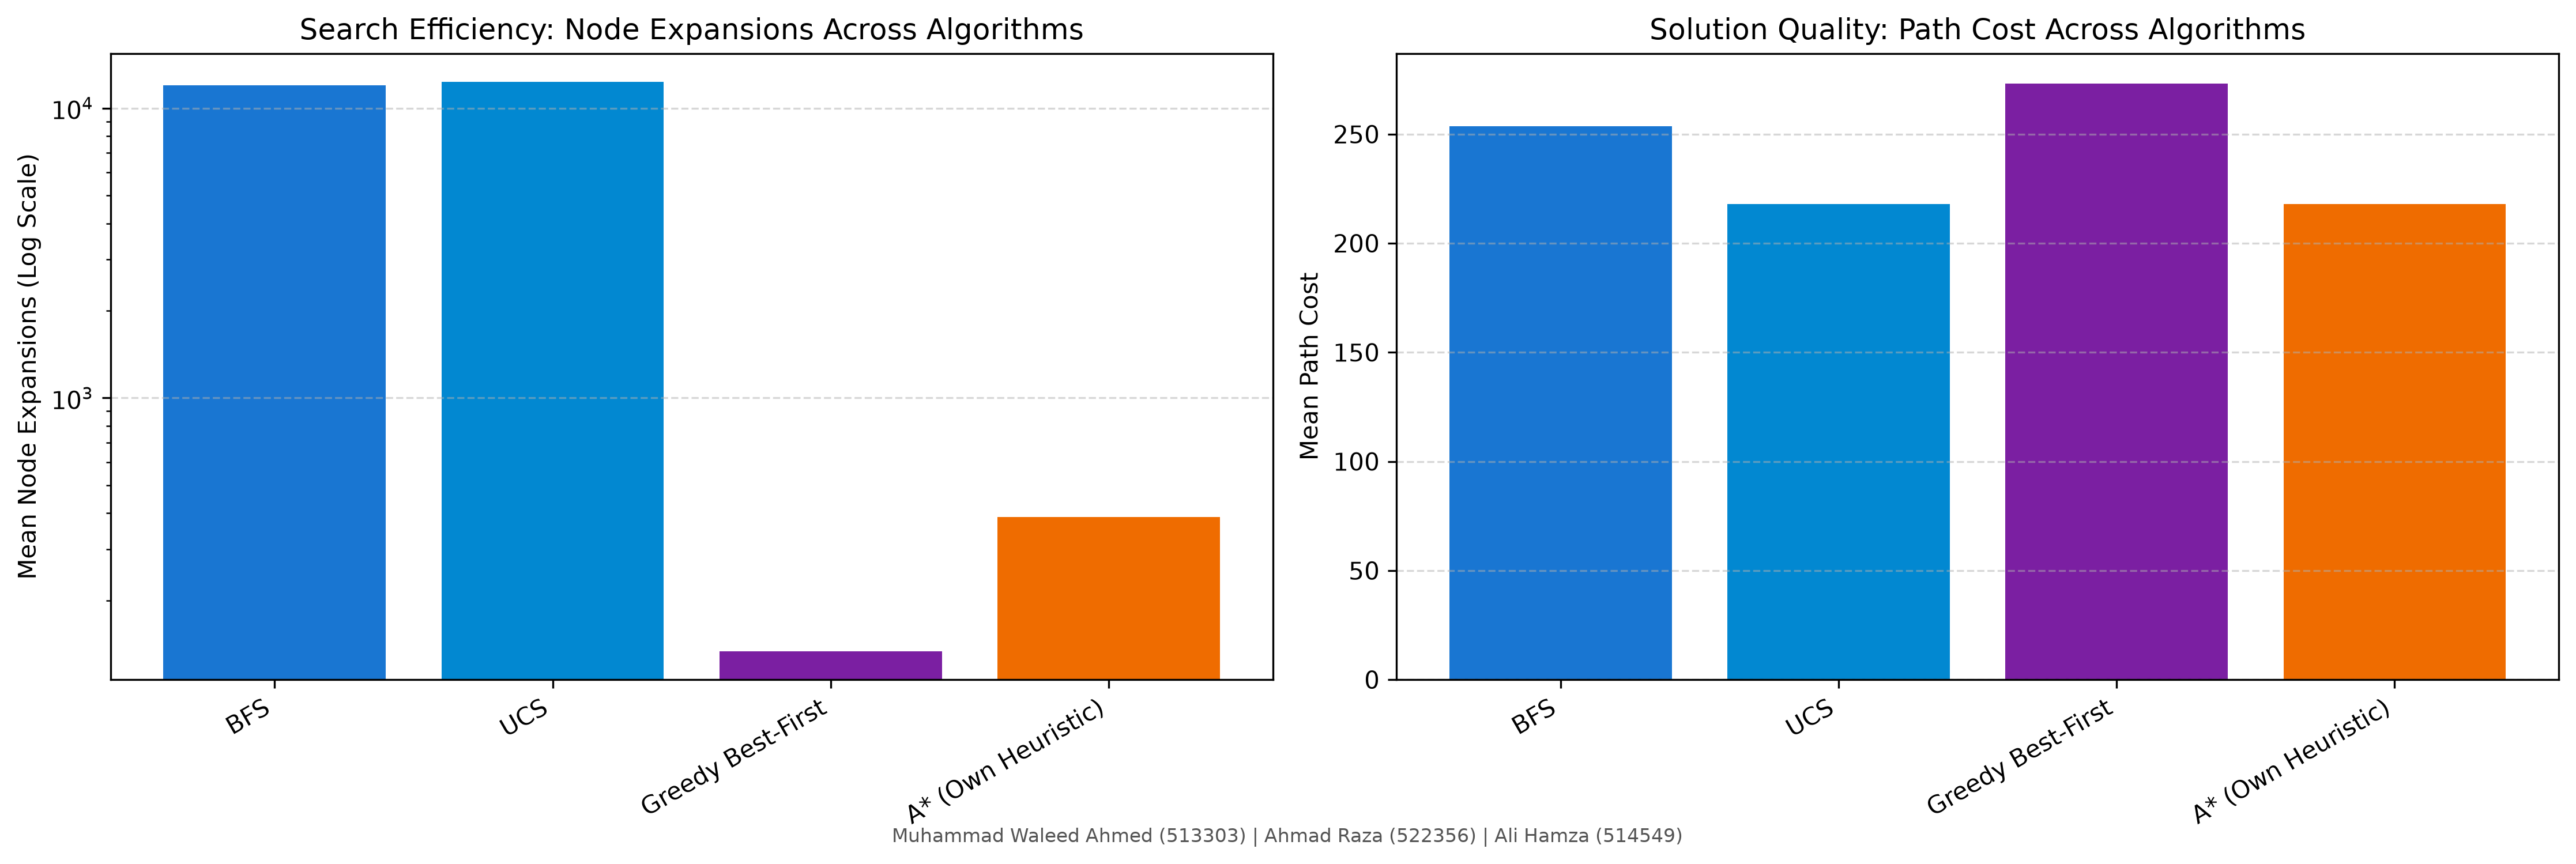
\includegraphics[width=0.90\columnwidth]{partB_six_algorithms_comparison.png}
    \caption{Six-algorithm comparison on solved ratio, expansions, and solution cost. | \stampline}
    \label{fig:six_algos}
\end{figure}

\begin{figure}[t]
    \centering
    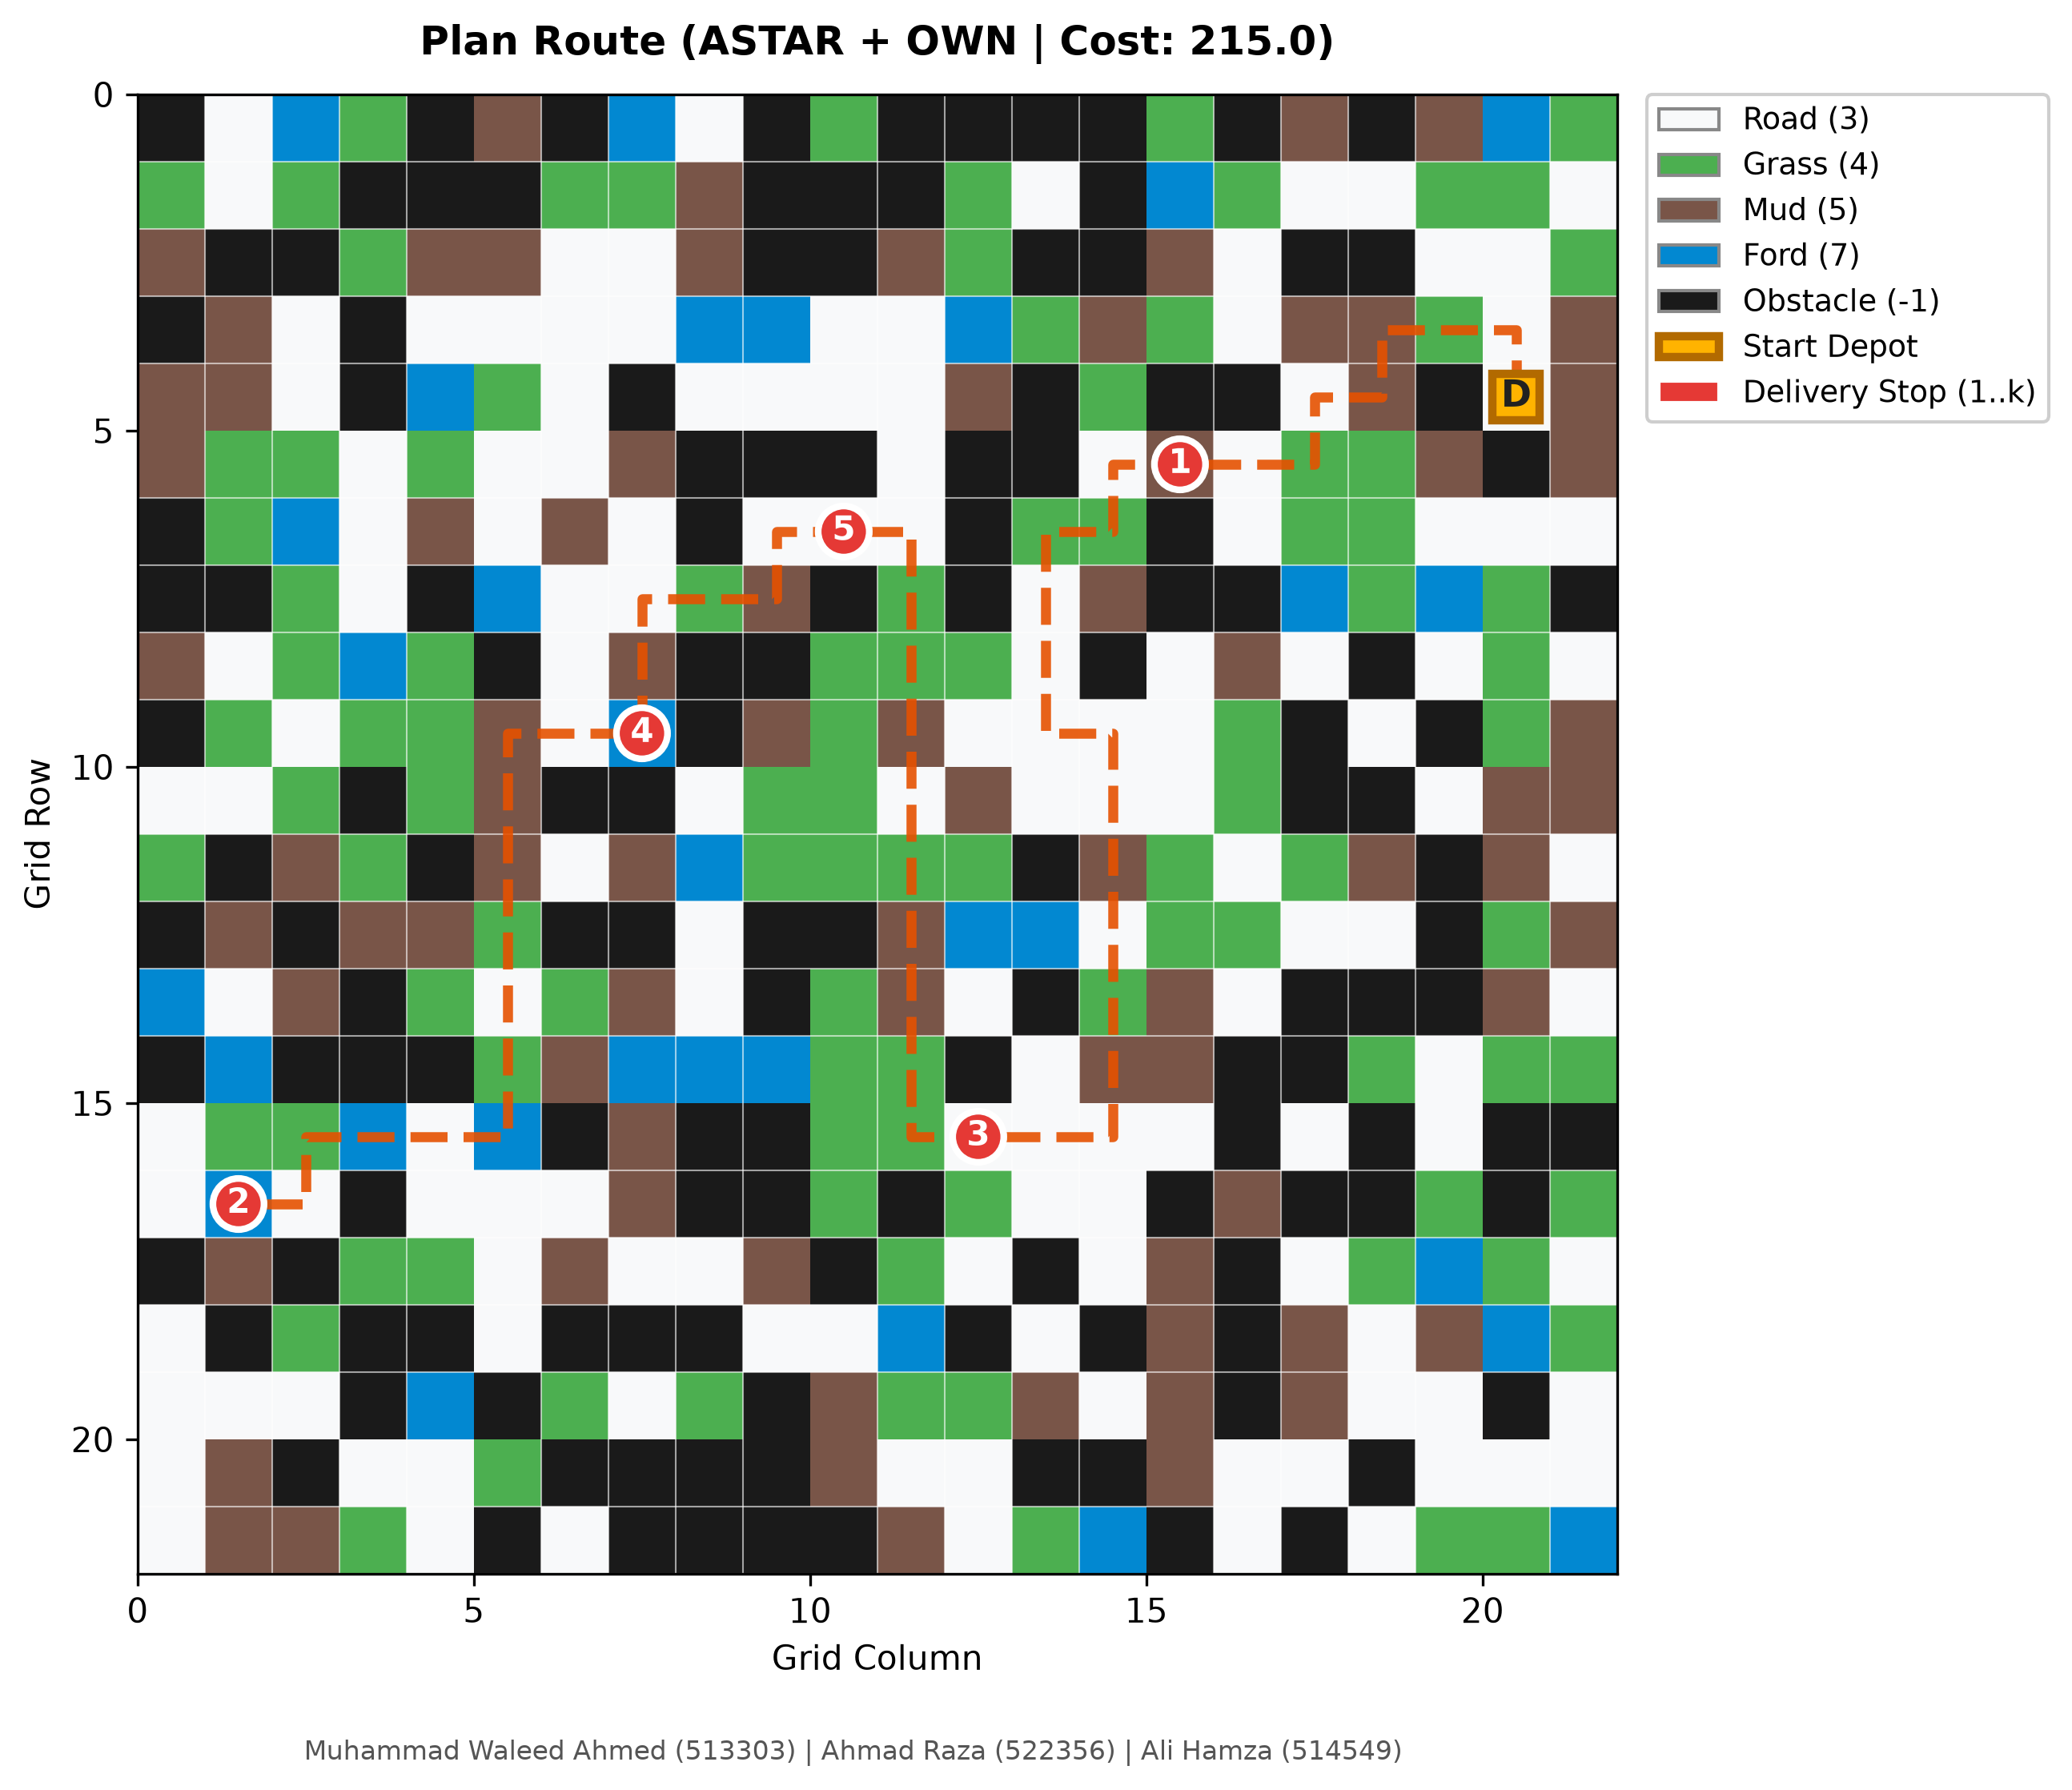
\includegraphics[width=0.90\columnwidth]{plan_astar_own.png}
    \caption{Optimal A* (\texttt{own}) delivery route on the canonical instance ($C=268.0$). | \stampline}
    \label{fig:plan_own}
\end{figure}

\subsection{Inadmissible Variant and Stored-Node Budget}
Using Weighted A* ($f = g + w \cdot h_{\text{own}}$) with $w > 1$ trades optimality for speed (Table~\ref{tab:inadmissible}): at $w=3.0$, node expansions drop by $40.6\%$ ($186.0$ vs.\ $387.4$) at the cost of a $5.68\%$ mean suboptimality gap (cost $230.23$ vs.\ $218.07$). Fig.~\ref{fig:inadmissible_showcase} shows a generated scenario where Weighted A* returns a suboptimal route. Under a tight stored-record budget of $25$ records (Table~\ref{tab:ids_budget}, Fig.~\ref{fig:ids_scaling}), BFS, UCS, and A* all fail ($0/5$) due to frontier/explored storage, whereas IDS with path-cycle avoidance solves $5/5$ using only $20.0$ peak stored records ($3.7$\,KB via \texttt{tracemalloc}). Path-cycle avoidance reduces IDS expansions from $6379$ to $898$ on the cycle ablation fixture.

\begin{table}[t]
    \centering
    \caption{Weighted A* Inadmissible Suboptimality Gap (30 Scenarios). | \stampline}
    \label{tab:inadmissible}
    \scriptsize
    \begin{tabular}{@{}rrrrr@{}}
        \toprule
        Weight $w$ & Expansions & Runtime (ms) & Mean Cost & Subopt.\ Gap \\
        \midrule
        1.0 (Optimal) & 387.4 & 23.21 & 218.07 & 0.00\% \\
        1.2           & 257.7 & 15.43 & 218.57 & 0.25\% \\
        1.5           & 232.5 & 14.74 & 219.77 & 0.84\% \\
        2.0           & 213.8 & 12.62 & 223.73 & 2.61\% \\
        3.0           & 186.0 & 11.33 & 230.23 & 5.68\% \\
        \bottomrule
    \end{tabular}
\end{table}

\begin{table}[t]
    \centering
    \caption{IDS vs.\ Graph Search Under a 25-Record Stored Budget. | \stampline}
    \label{tab:ids_budget}
    \scriptsize
    \begin{tabular}{@{}lrrrr@{}}
        \toprule
        Algorithm (Budget=25) & Solved & Peak Stored & Peak Mem (KB) & Expansions \\
        \midrule
        BFS      & 0/5 & 26.2 & 5.0 & DNF \\
        UCS      & 0/5 & 26.6 & 2.4 & DNF \\
        A* (Own) & 0/5 & 28.0 & 3.6 & DNF \\
        IDS      & 5/5 & 20.0 & 3.7 & 3212.4 \\
        \bottomrule
    \end{tabular}
\end{table}

\begin{figure}[t]
    \centering
    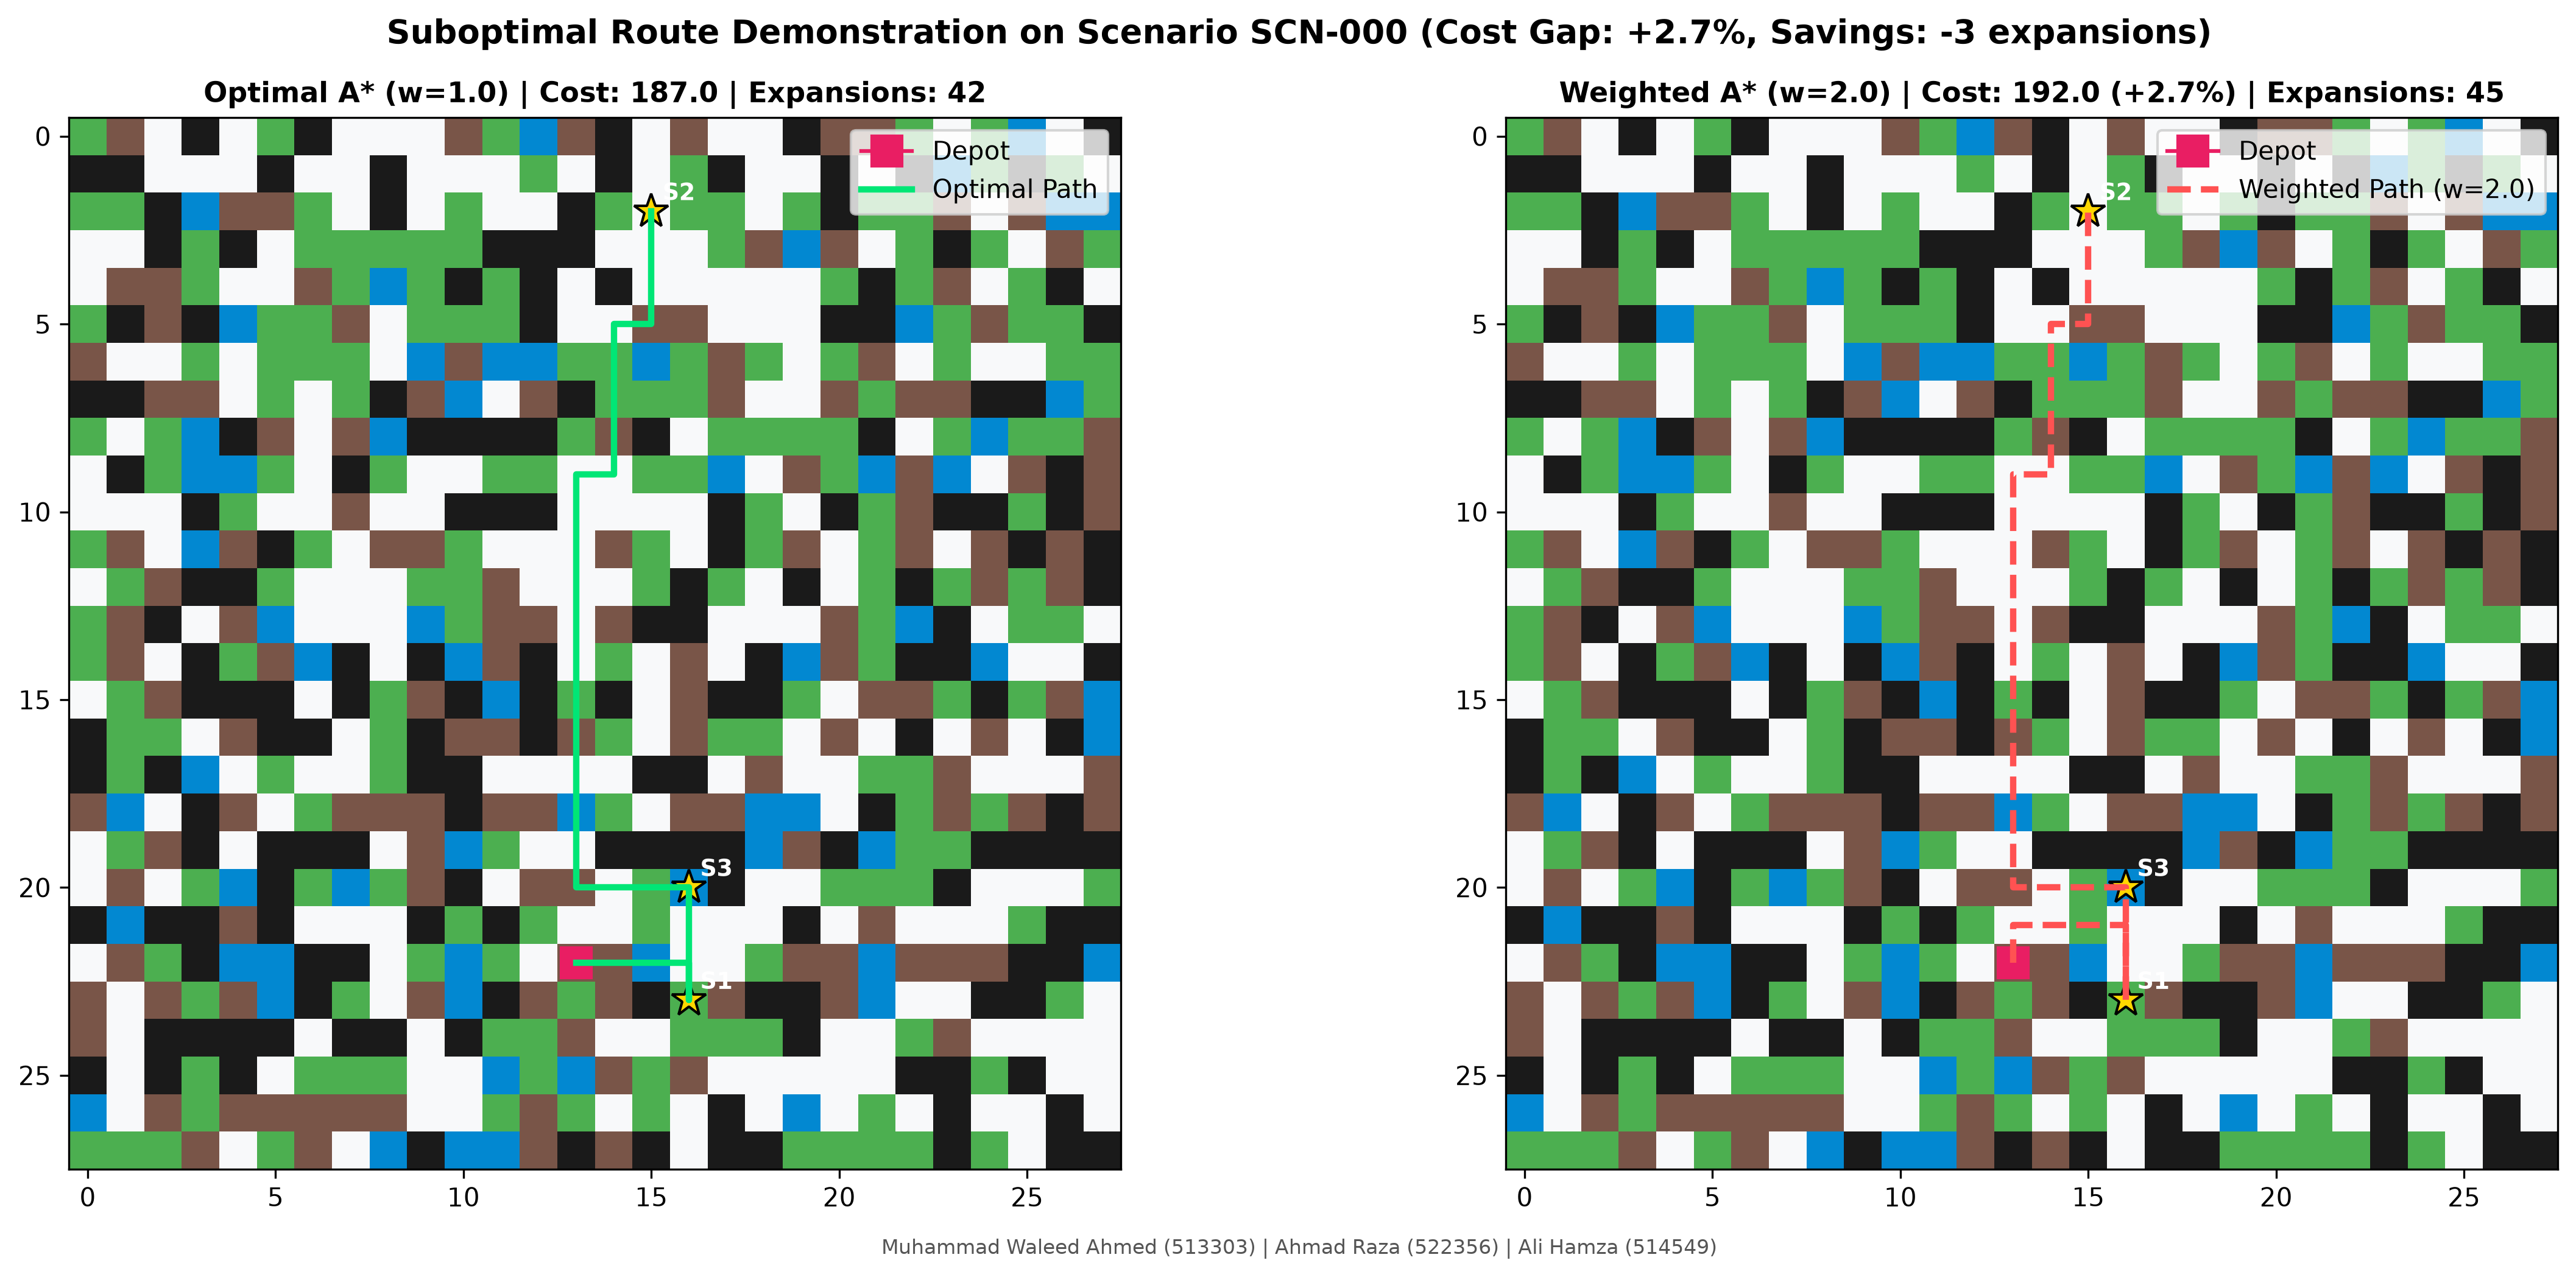
\includegraphics[width=0.90\columnwidth]{partB_inadmissible_suboptimal_showcase.png}
    \caption{Suboptimal route returned by Weighted A* ($w > 1$) vs.\ optimal A*. | \stampline}
    \label{fig:inadmissible_showcase}
\end{figure}

\begin{figure}[t]
    \centering
    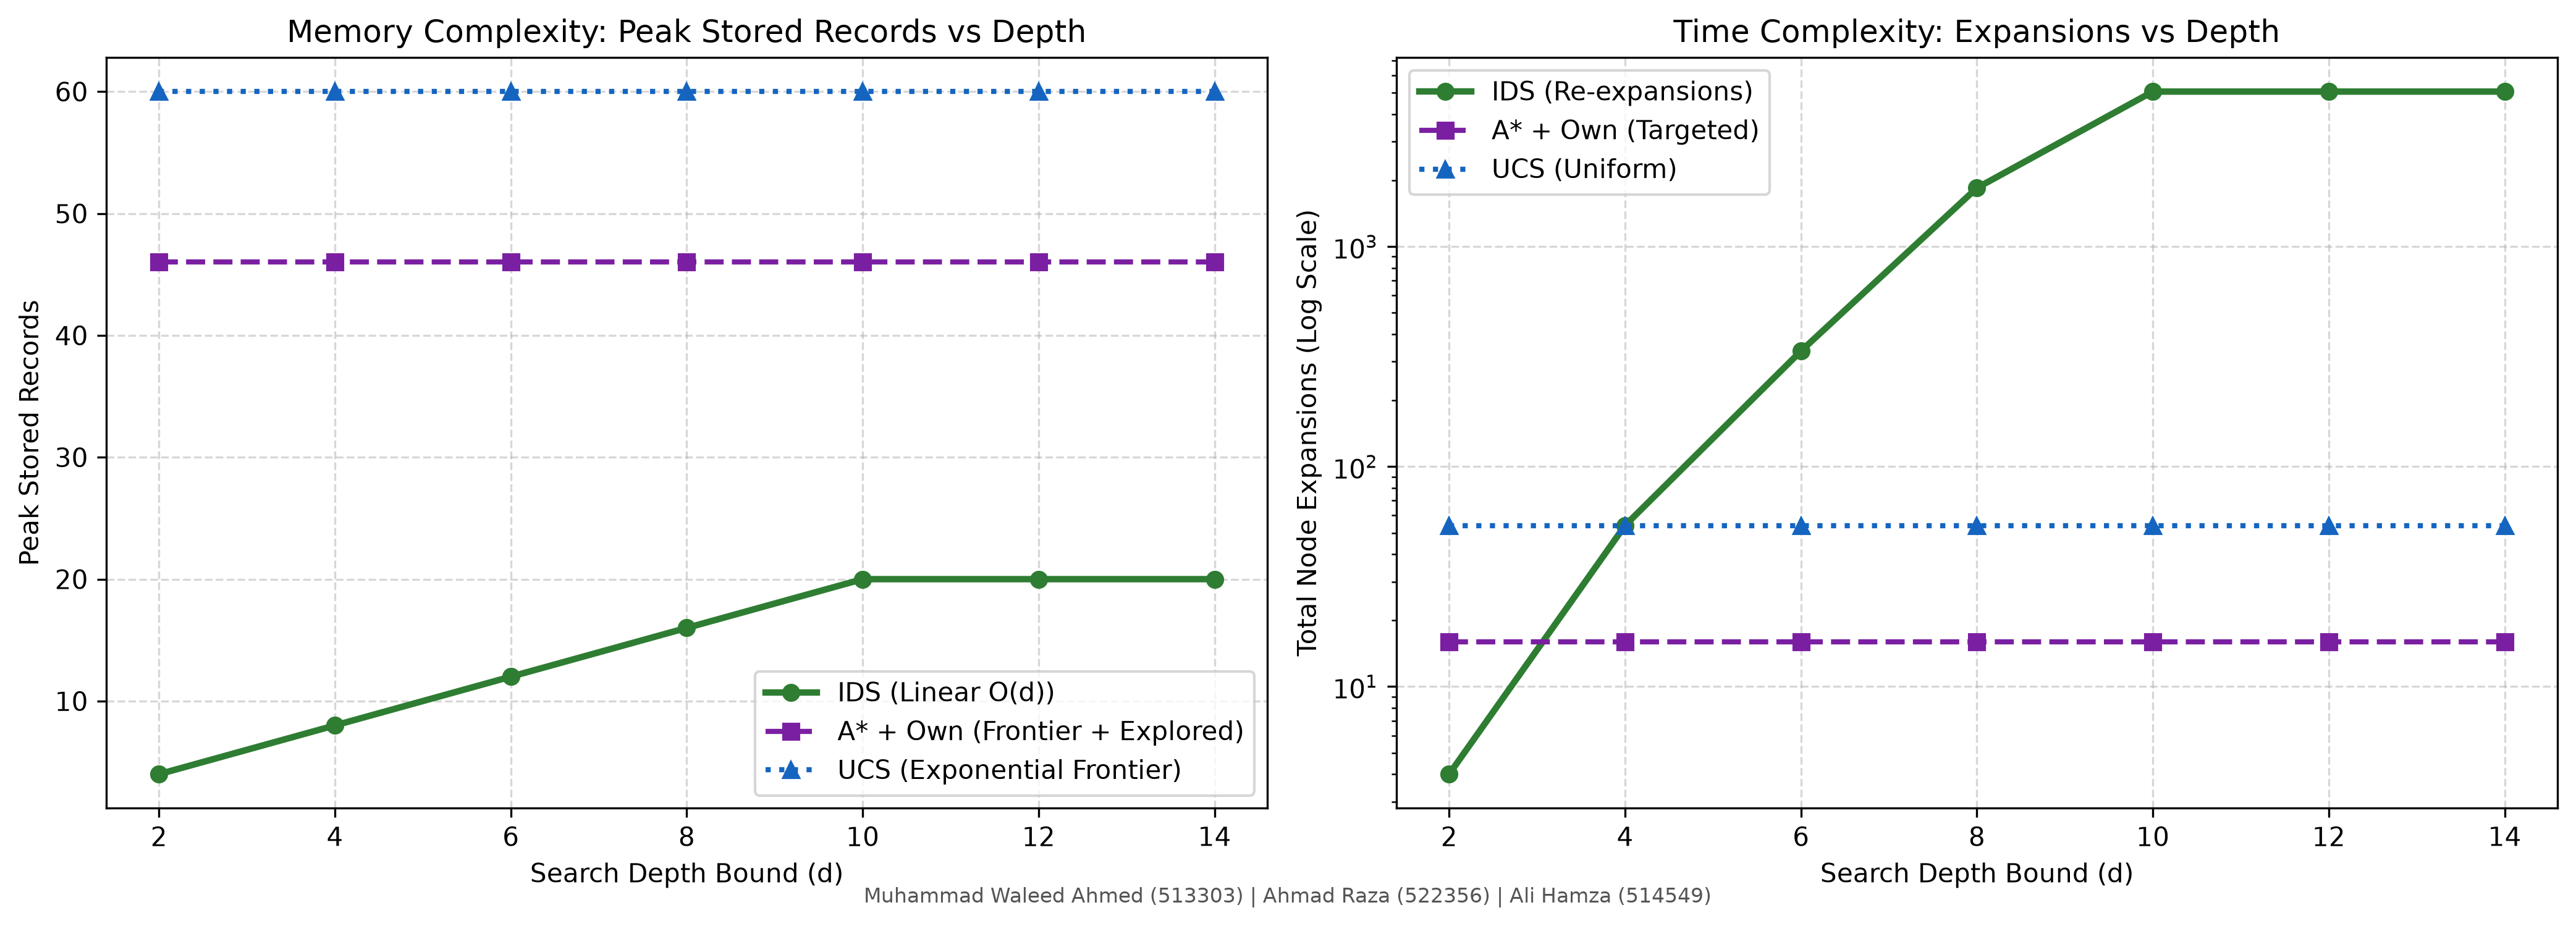
\includegraphics[width=0.90\columnwidth]{partB_ids_scaling_curves.png}
    \caption{IDS vs.\ A*/UCS/BFS under stored-record budget constraints. | \stampline}
    \label{fig:ids_scaling}
\end{figure}

\section{Part C: Adversarial Rival and Stochastic Execution}
\subsection{Reduced Game and Alpha-Beta Pruning}
We model the interaction against the \texttt{chaser} rival on a reduced local square window of Chebyshev radius $r=4$ around the courier, with action set $\{N, E, S, W, \text{WAIT}\}$ and alternating plies up to depth $6$. Terminal precedence evaluates capture first (Loss), then all-stops delivered with $C \le \kappa C^*$ ($\kappa=1.5$, Win) or $C > \kappa C^*$ (Draw), then step cap $T_{\max} = 4L^* + 20$ (Draw).

Across \numPartcPruningPositions{} non-terminal game positions sampled from 30 scenarios (Table~\ref{tab:pruning}, Fig.~\ref{fig:pruning}), Alpha-Beta \cite{knuth1975alphabeta} with our custom move ordering (prioritising delivery-progress and safe moves) produces zero value mismatches against Minimax while cutting depth-6 evaluations from $2293.8$ to \numPartcPruningDSixOwnEvals{}—a \numPartcPruningDSixSavedMmPct{}\% reduction versus Minimax and $44.6\%$ versus natural-order Alpha-Beta.

\begin{table}[t]
    \centering
    \caption{Minimax vs.\ Alpha-Beta Evaluations Across \numPartcPruningPositions{} Positions. | \stampline}
    \label{tab:pruning}
    \scriptsize
    \begin{tabular}{@{}rlrrr@{}}
        \toprule
        Depth & Ordering & Minimax & Alpha-Beta (95\% CI) & Saved vs.\ MM \\
        \midrule
        2 & own & 14.1   & 7.6 [7.3, 8.0]       & 42.4\% \\
        3 & own & 54.9   & 18.6 [17.6, 19.6]    & 62.6\% \\
        4 & own & 216.7  & 31.7 [29.9, 33.5]    & 81.4\% \\
        5 & own & 609.8  & 79.7 [73.9, 85.6]    & 84.1\% \\
        6 & natural & 2293.8 & 481.3 [418.5, 544.2] & 80.2\% \\
        6 & own & 2293.8 & \numPartcPruningDSixOwnEvals{} [126.5, 148.3] & \numPartcPruningDSixSavedMmPct{}\% \\
        \bottomrule
    \end{tabular}
\end{table}

\begin{figure}[t]
    \centering
    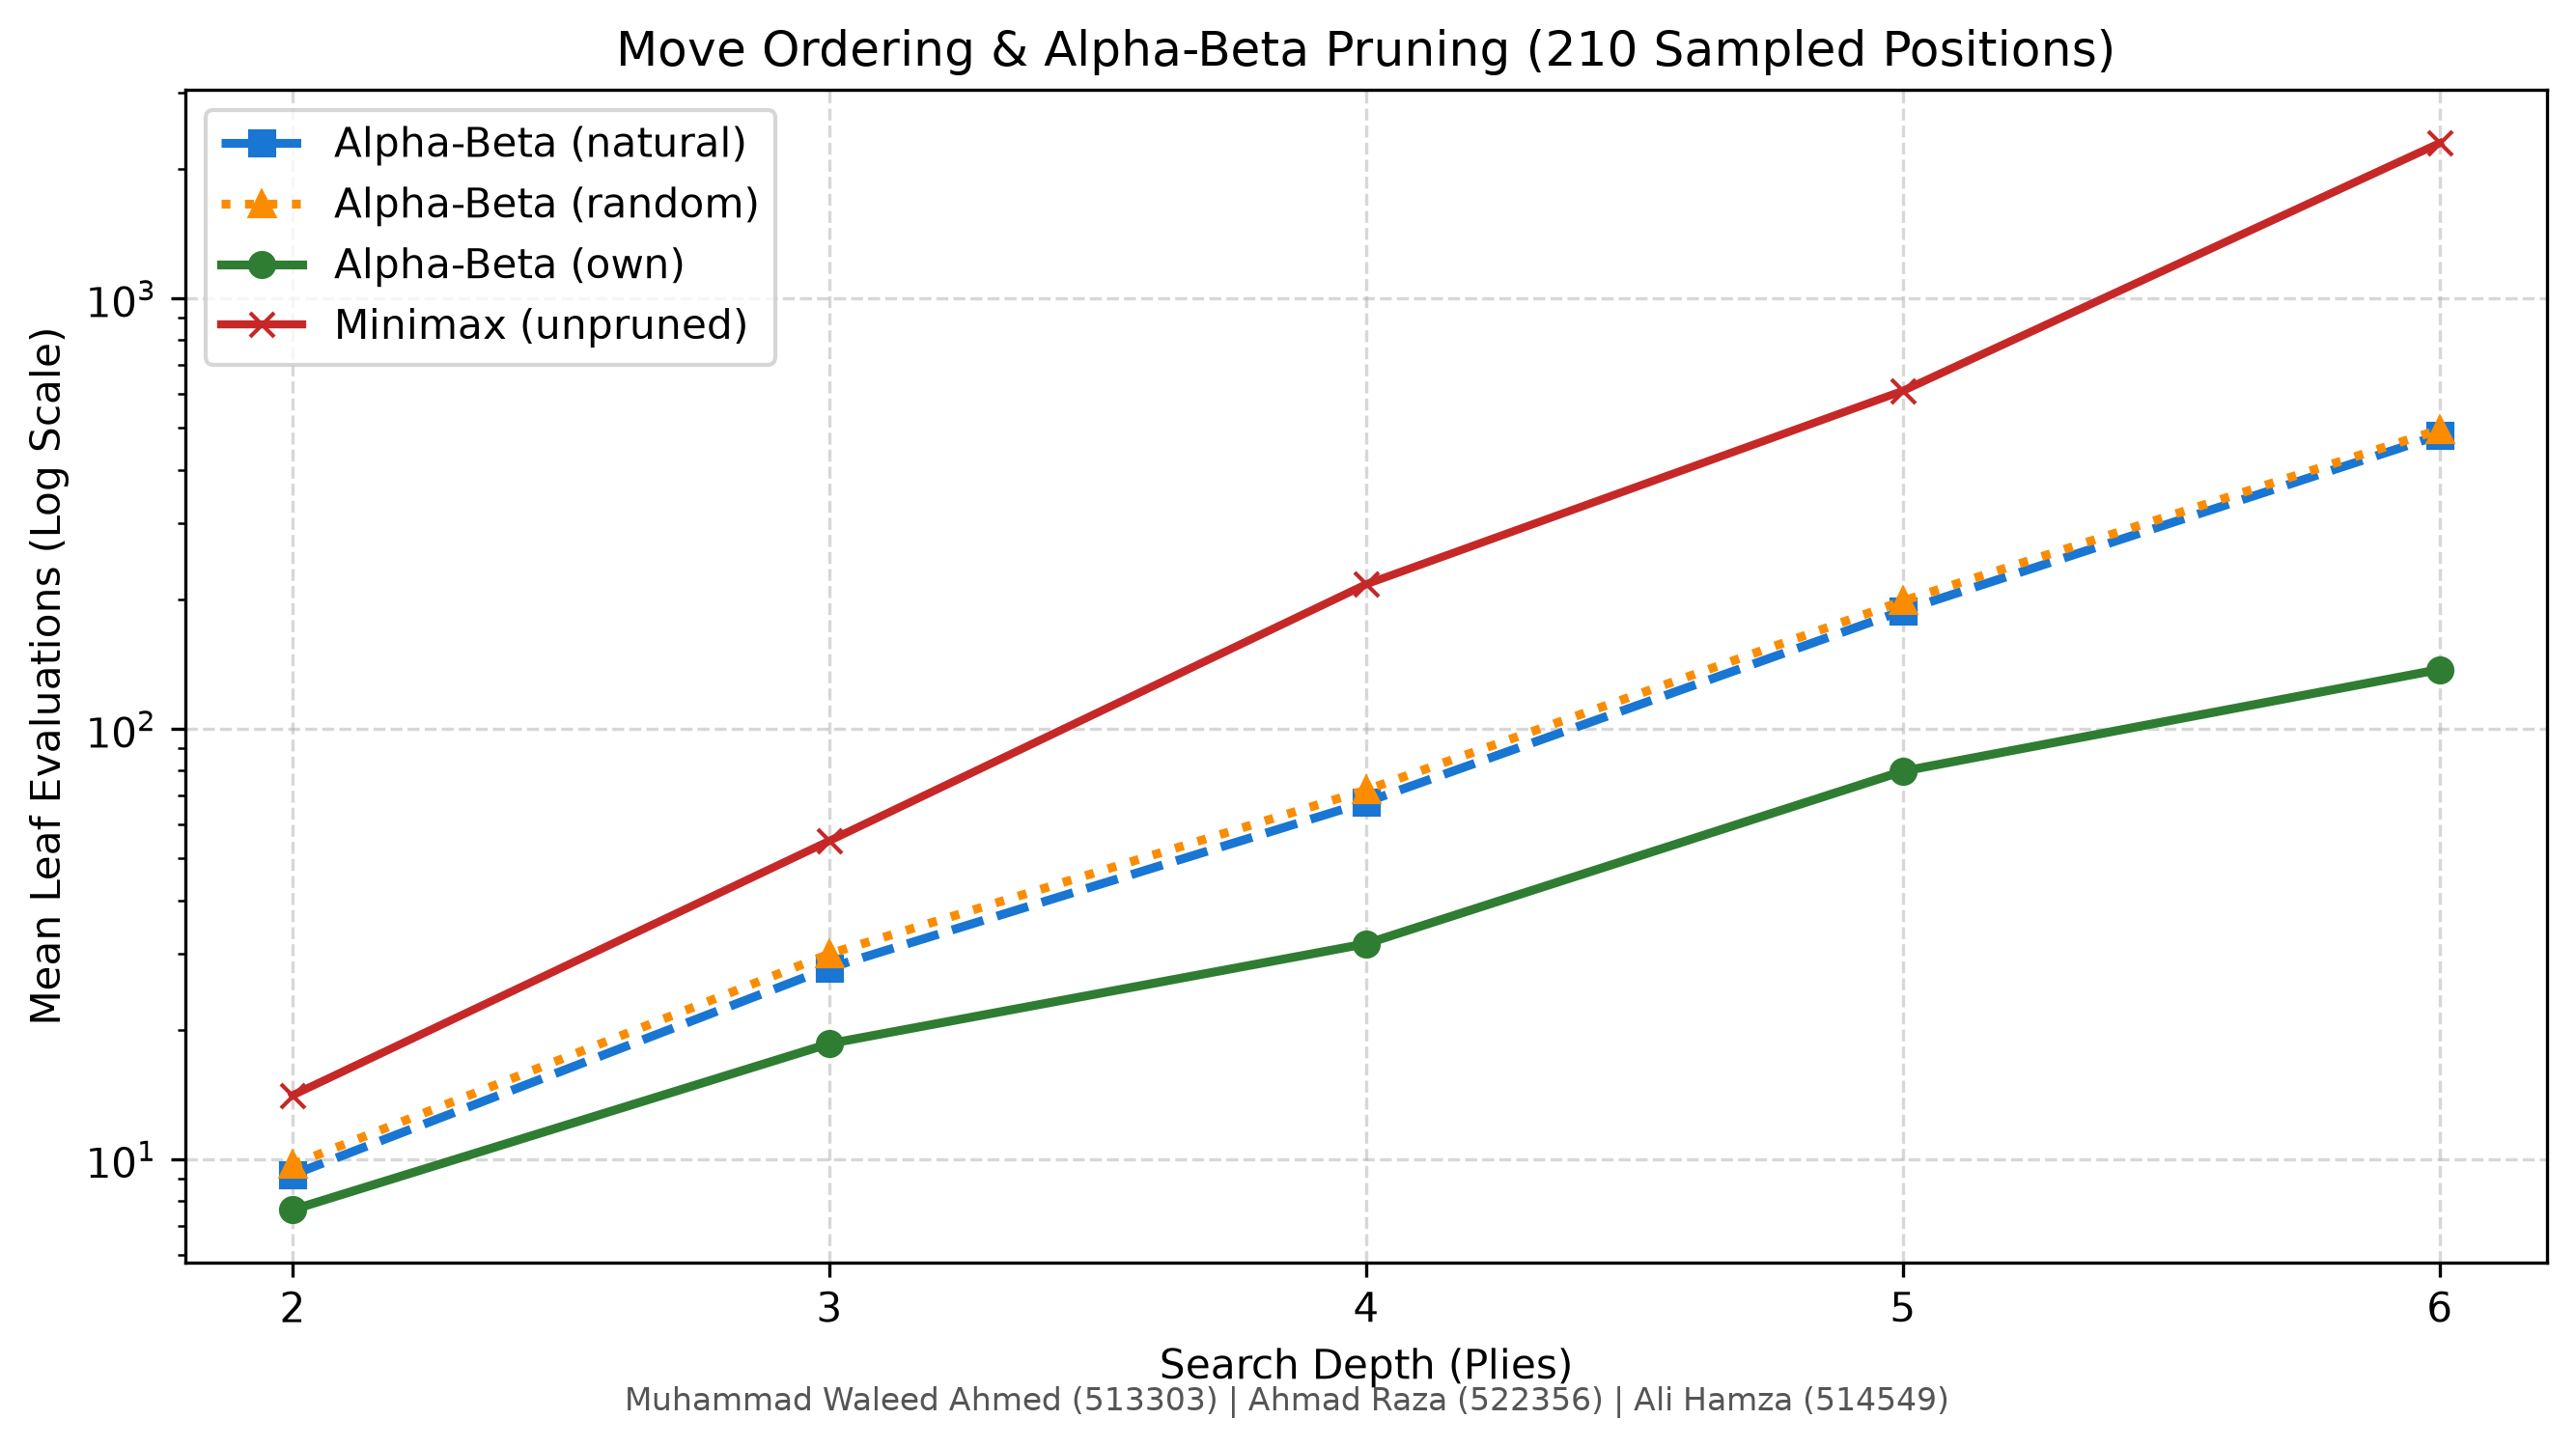
\includegraphics[width=0.90\columnwidth]{partC_pruning_curves.png}
    \caption{Alpha-Beta evaluation savings vs.\ Minimax across depths $2$--$6$. | \stampline}
    \label{fig:pruning}
\end{figure}

\subsection{Slip Dynamics and Deterministic Model Mismatch}
Our hybrid agent pairs global A* planning with local depth-6 Alpha-Beta tactical lookahead, replanning after every realised slip or rival divergence. Both A* and Alpha-Beta assume deterministic transitions, whereas the simulator applies slip $p$. Table~\ref{tab:slip} and Fig.~\ref{fig:slip} show a paired 15-scenario sweep across $p \in \{0.0, 0.1, 0.2, 0.23, 0.3, 0.5\}$: at $p=0.5$, win rate drops from $26.7\%$ to $6.7\%$ and replan frequency climbs to $66.2$ replans per 100 moves.

\begin{table}[t]
    \centering
    \caption{Stochastic Slip Sweep Across 15 Paired Scenarios. | \stampline}
    \label{tab:slip}
    \scriptsize
    \begin{tabular}{@{}rrrrr@{}}
        \toprule
        Slip $p$ & Win Rate (95\% CI) & Capture Rate & Replans/100 & Mean Cost \\
        \midrule
        0.00 & 26.7\% [10.9, 52.0] & 60.0\% & 52.9 & 336.3 \\
        0.10 & 20.0\% [7.0, 45.2]  & 73.3\% & 41.8 & 246.6 \\
        0.20 & 13.3\% [3.7, 37.9]  & 80.0\% & 46.8 & 250.7 \\
        0.23 & 13.3\% [3.7, 37.9]  & 80.0\% & 49.0 & 251.5 \\
        0.30 & 13.3\% [3.7, 37.9]  & 80.0\% & 51.2 & 242.3 \\
        0.50 & 6.7\% [1.2, 29.8]   & 73.3\% & 66.2 & 321.2 \\
        \bottomrule
    \end{tabular}
\end{table}

\begin{figure}[t]
    \centering
    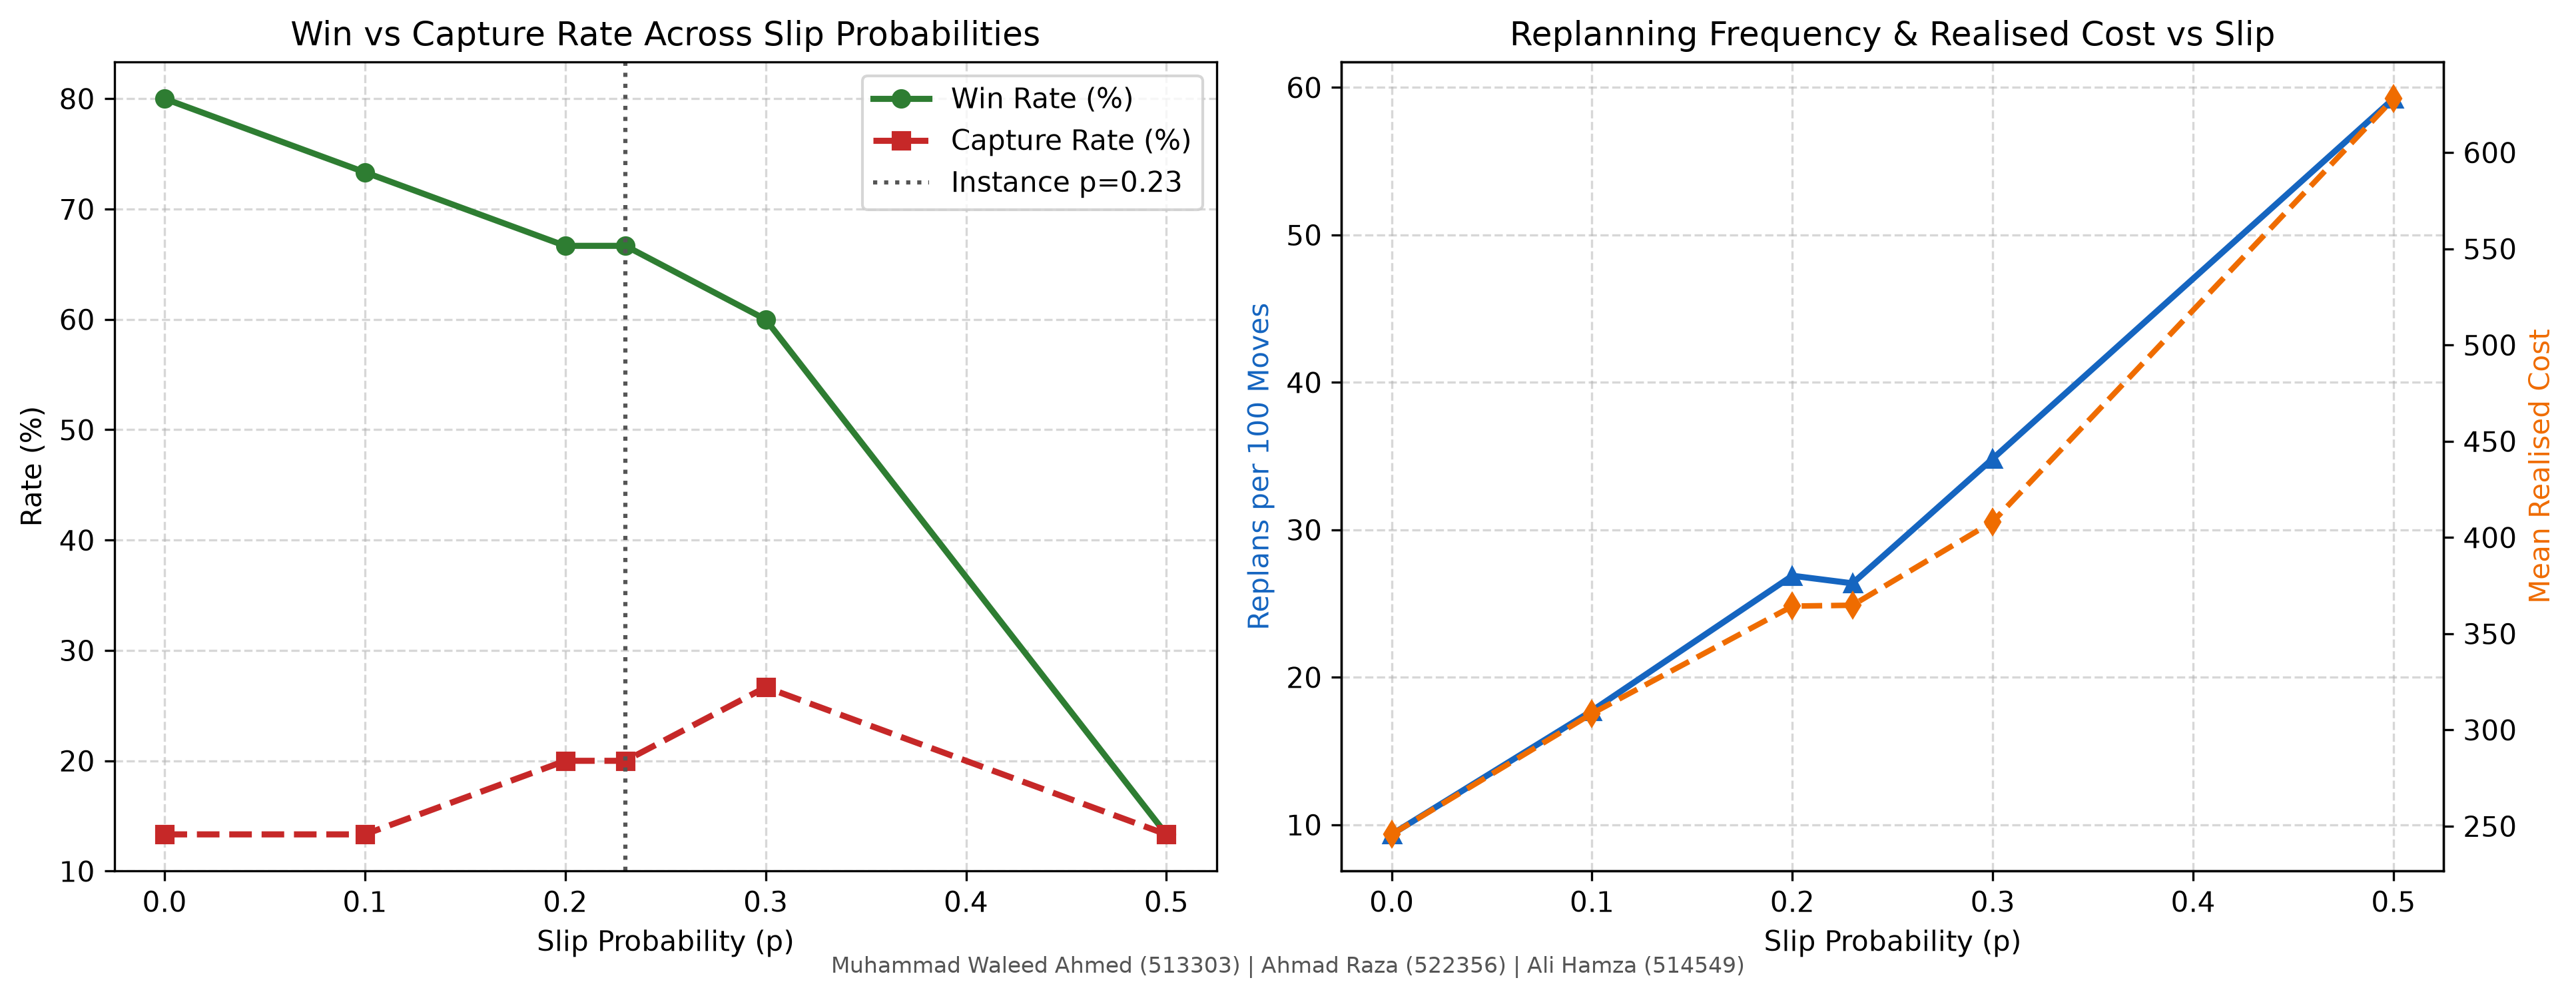
\includegraphics[width=0.90\columnwidth]{partC_slip_analysis.png}
    \caption{Impact of slip probability $p$ on win rate, capture rate, and replan frequency. | \stampline}
    \label{fig:slip}
\end{figure}

\subsection{Evaluation Function, Weight Tuning, and 50-Game Results}
Non-terminal game states are scored by a 4-feature linear evaluation: (1) delivered-stop progress bonus, (2) negative remaining relaxed MST distance, (3) obstacle-aware reverse-BFS rival-distance safety margin, and (4) local terrain/cost penalty. Grid-search tuning on disjoint tuning seeds (Fig.~\ref{fig:tuning}) selected route-heavy weights. Across \numPartcGamesCount{} evaluation games against the \texttt{chaser} (Table~\ref{tab:games}), both Default and Tuned weights achieved \numPartcTunedWinPct{}\% wins ($[2.1\%, 16.2\%]$), $6.0\%$ draws, and $88.0\%$ captures, with mean cost \numPartcDefaultMeanCost{} (Default) vs.\ \numPartcTunedMeanCost{} (Tuned)—reflecting the intrinsic difficulty of evading an omniscient depth-6 \texttt{chaser} under $p=0.23$ slip and one-way constraints (Fig.~\ref{fig:replay_win}).

\begin{table}[t]
    \centering
    \caption{Final \numPartcGamesCount{}-Game Evaluation vs.\ \texttt{chaser} ($p=0.23$). | \stampline}
    \label{tab:games}
    \scriptsize
    \begin{tabular}{@{}lrrrrr@{}}
        \toprule
        Config & Win Rate (95\% CI) & Draw Rate & Loss Rate & Mean Cost & Replans \\
        \midrule
        Default & \numPartcTunedWinPct{}\% [2.1, 16.2] & 6.0\% & 88.0\% & \numPartcDefaultMeanCost{} & 30.1 \\
        Tuned   & \numPartcTunedWinPct{}\% [2.1, 16.2] & 6.0\% & 88.0\% & \numPartcTunedMeanCost{}   & 30.8 \\
        \bottomrule
    \end{tabular}
\end{table}

\begin{figure}[t]
    \centering
    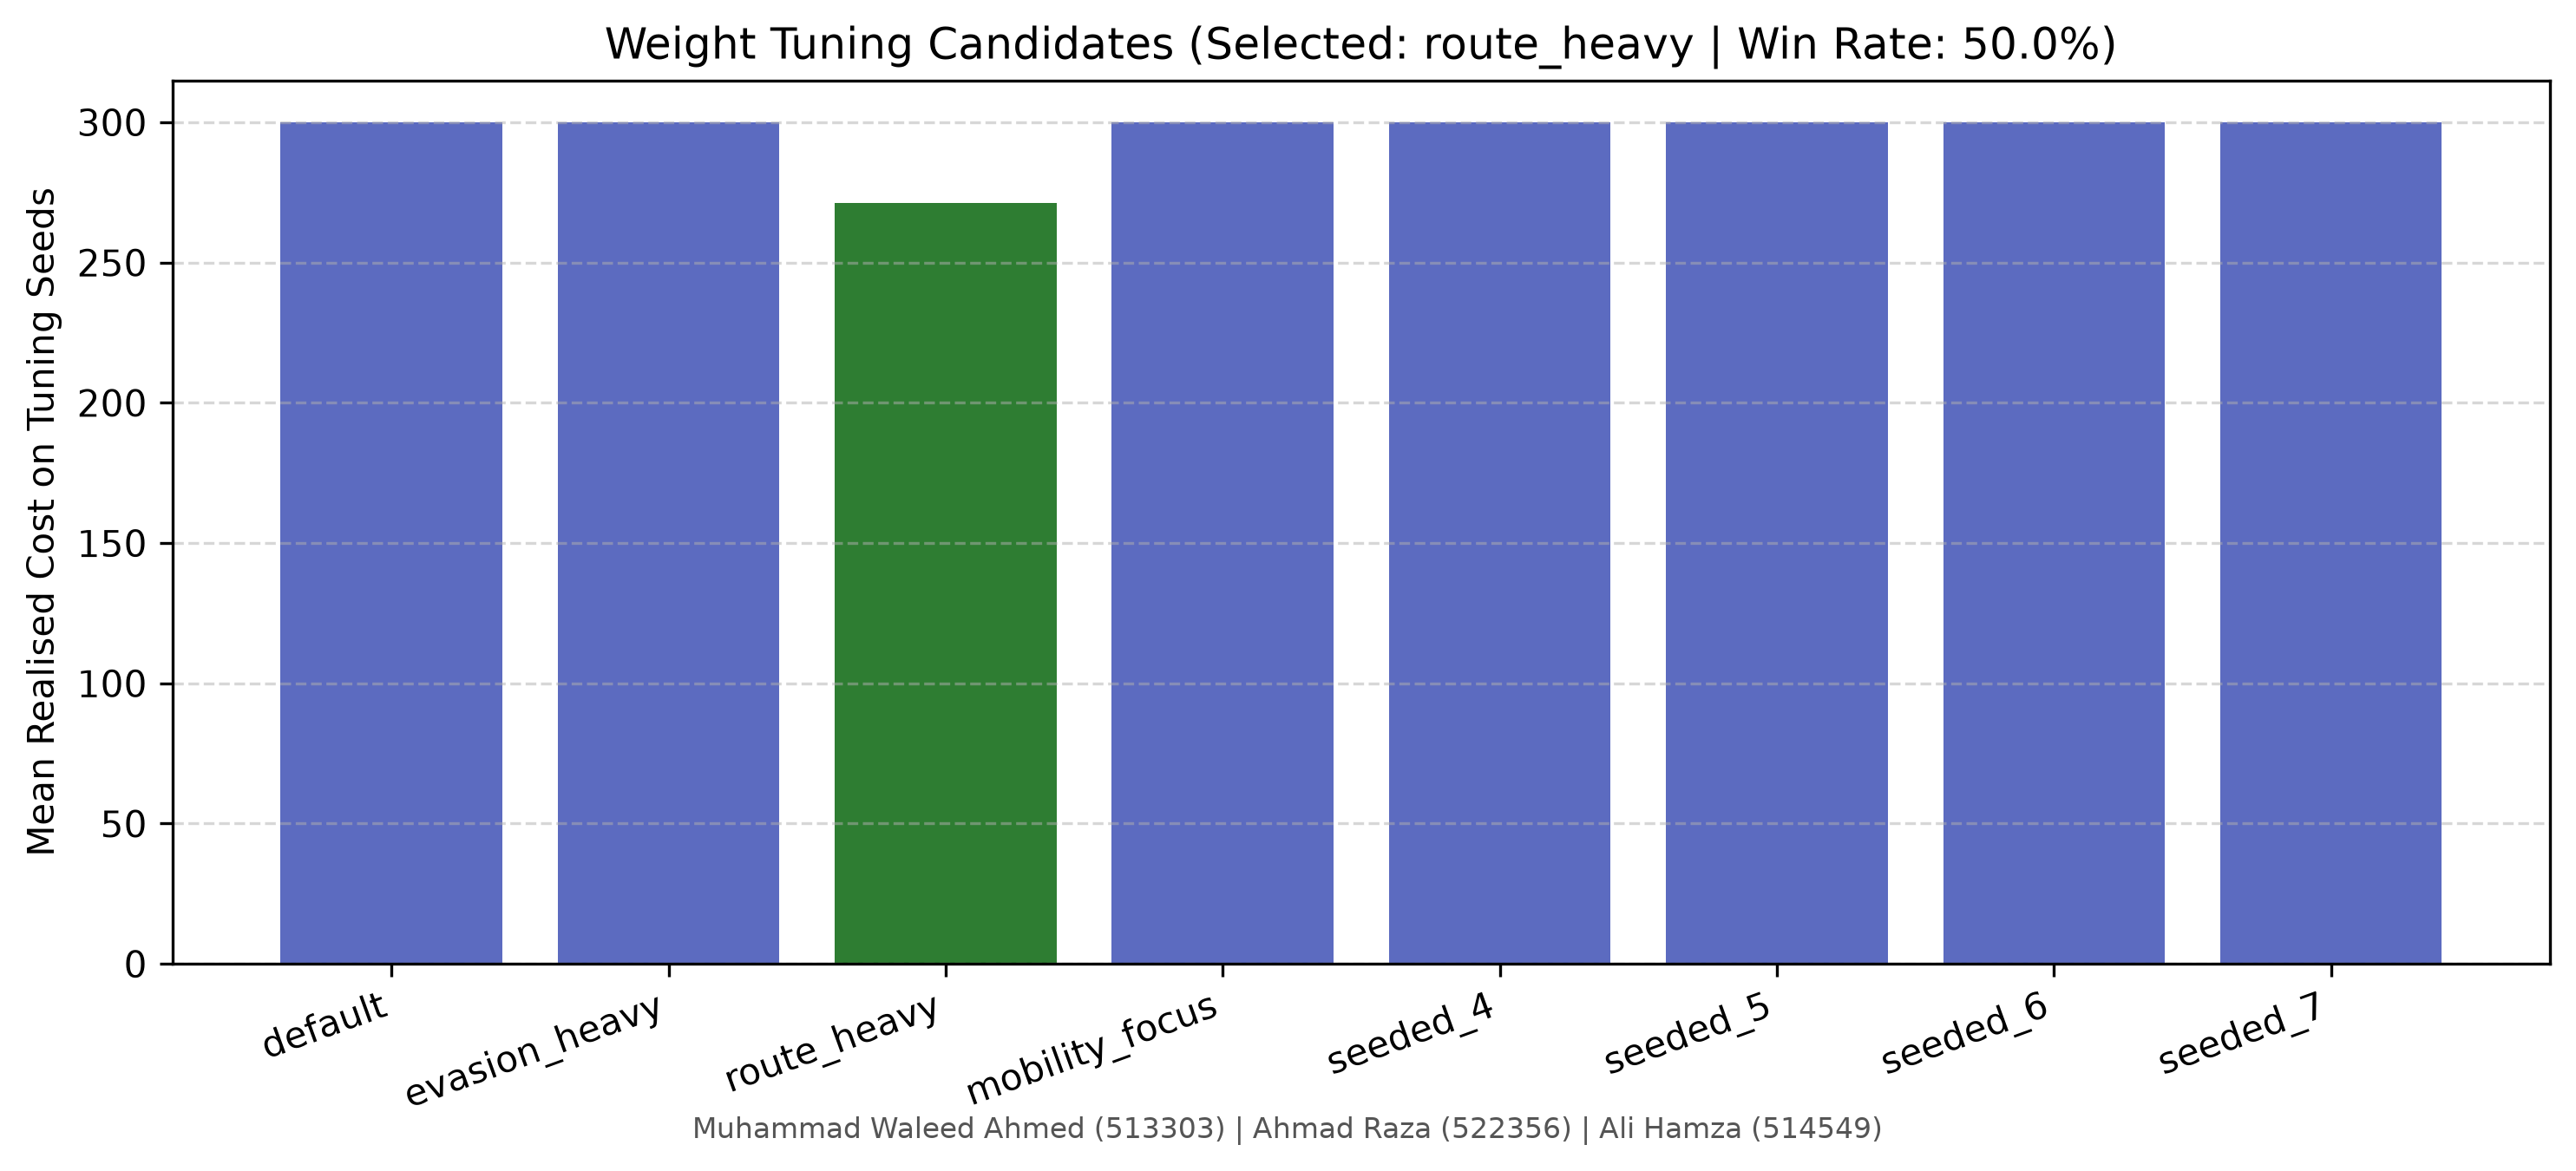
\includegraphics[width=0.90\columnwidth]{partC_tuning_comparison.png}
    \caption{Grid-search evaluation weight tuning on disjoint tuning scenarios. | \stampline}
    \label{fig:tuning}
\end{figure}

\begin{figure}[t]
    \centering
    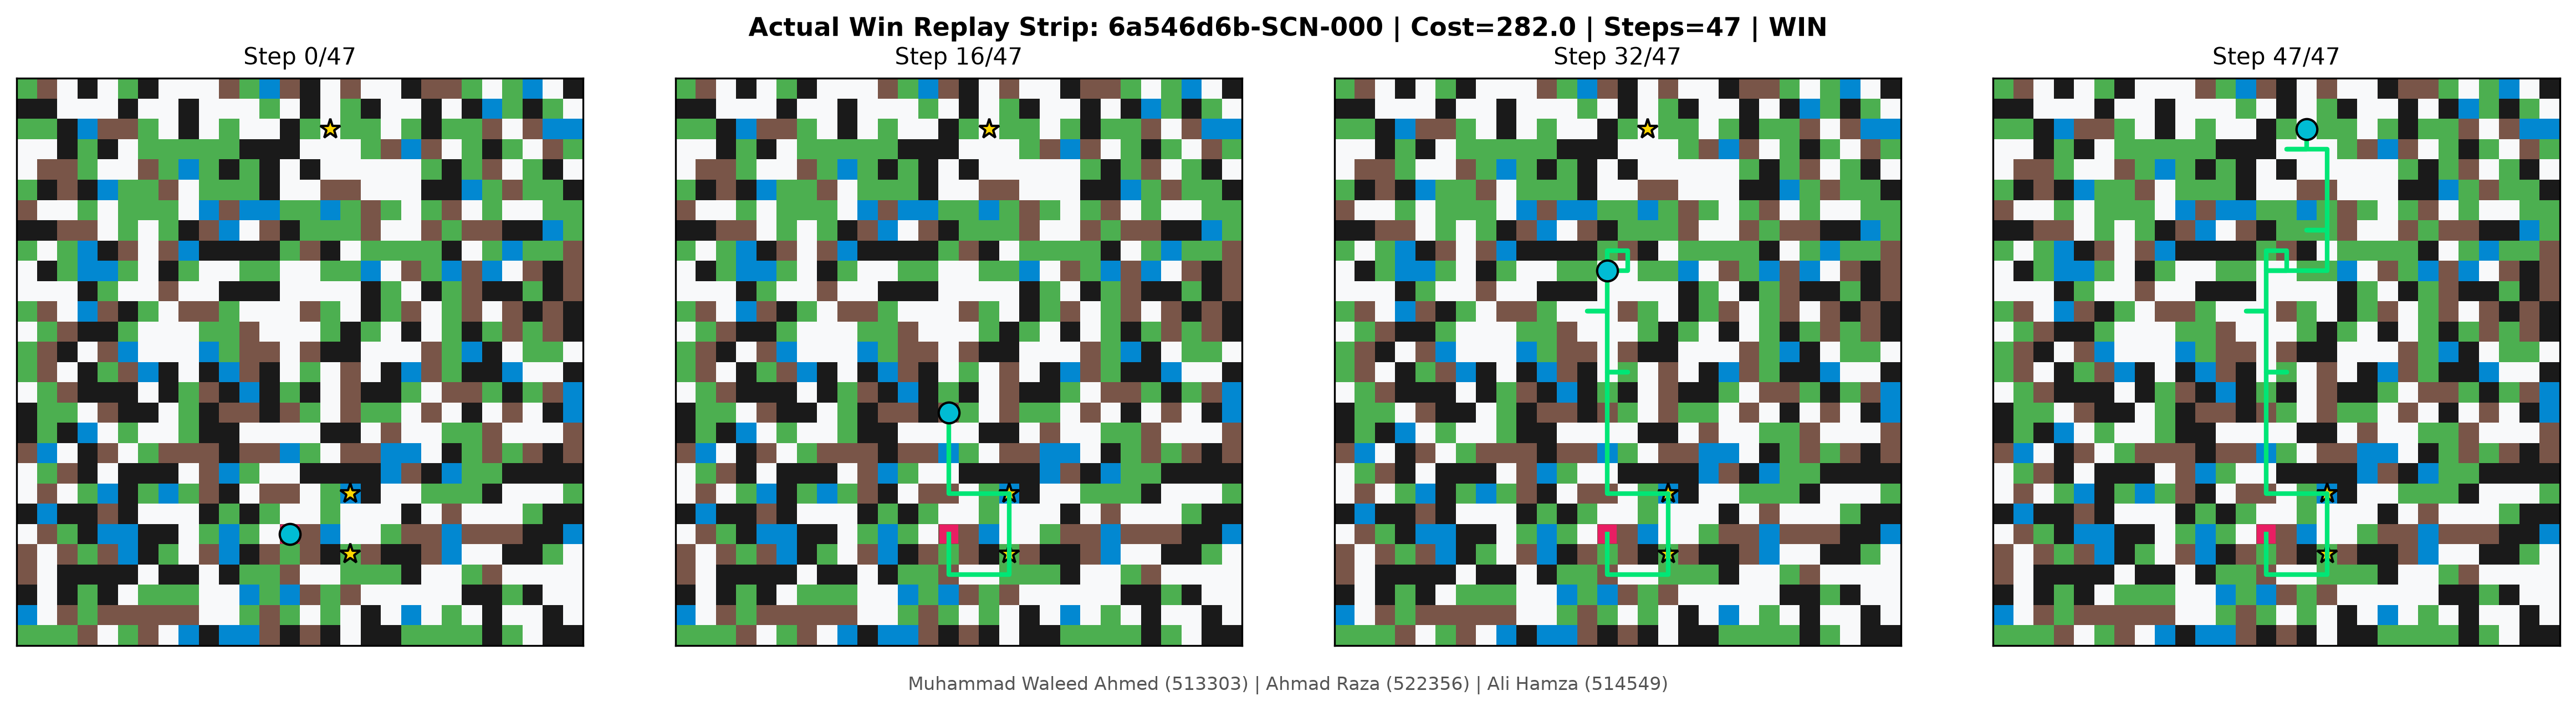
\includegraphics[width=0.90\columnwidth]{partC_replay_win.png}
    \caption{Sample winning game trajectory against the \texttt{chaser} rival. | \stampline}
    \label{fig:replay_win}
\end{figure}

\section{Part D: LLM Dispatcher}
We implemented a custom ReAct loop \cite{yao2023react} over a provider-agnostic \texttt{LLMClient} ($\text{temperature}=0.0$) equipped with \texttt{plan\_route}, \texttt{simulate}, and twist-specific inspection tools (\texttt{inspect\_twists}, \texttt{scan\_fog}). We evaluated \numPartdRequests{} natural-language requests spanning single-constraint, multi-constraint, twist-specific, ambiguous, and conflicting/infeasible categories on \texttt{groq/openai/gpt-oss-120b} (Table~\ref{tab:partd}, Fig.~\ref{fig:partd}).

\begin{table}[t]
    \centering
    \caption{Part D LLM Dispatcher vs.\ Direct Planner (\numPartdRequests{} Requests). | \stampline}
    \label{tab:partd}
    \scriptsize
    \begin{tabular}{@{}lrrrr@{}}
        \toprule
        Mode & Success (95\% Wilson CI) & Tool Acc. & Cost Ratio & Latency (s) \\
        \midrule
        Direct Planner      & 100.0\% [83.9, 100.0] & 100.0\% & 1.000 & 0.01 \\
        ReAct NoValidation  & \numPartdNovalSuccessPct{}\% [43.3, 81.9]   & 80.0\%  & 0.915 & 2.02 \\
        ReAct WithValidation& \numPartdWithvalSuccessPct{}\% [48.1, 85.5] & 85.0\%  & 0.857 & 2.06 \\
        \bottomrule
    \end{tabular}
\end{table}

\begin{figure}[t]
    \centering
    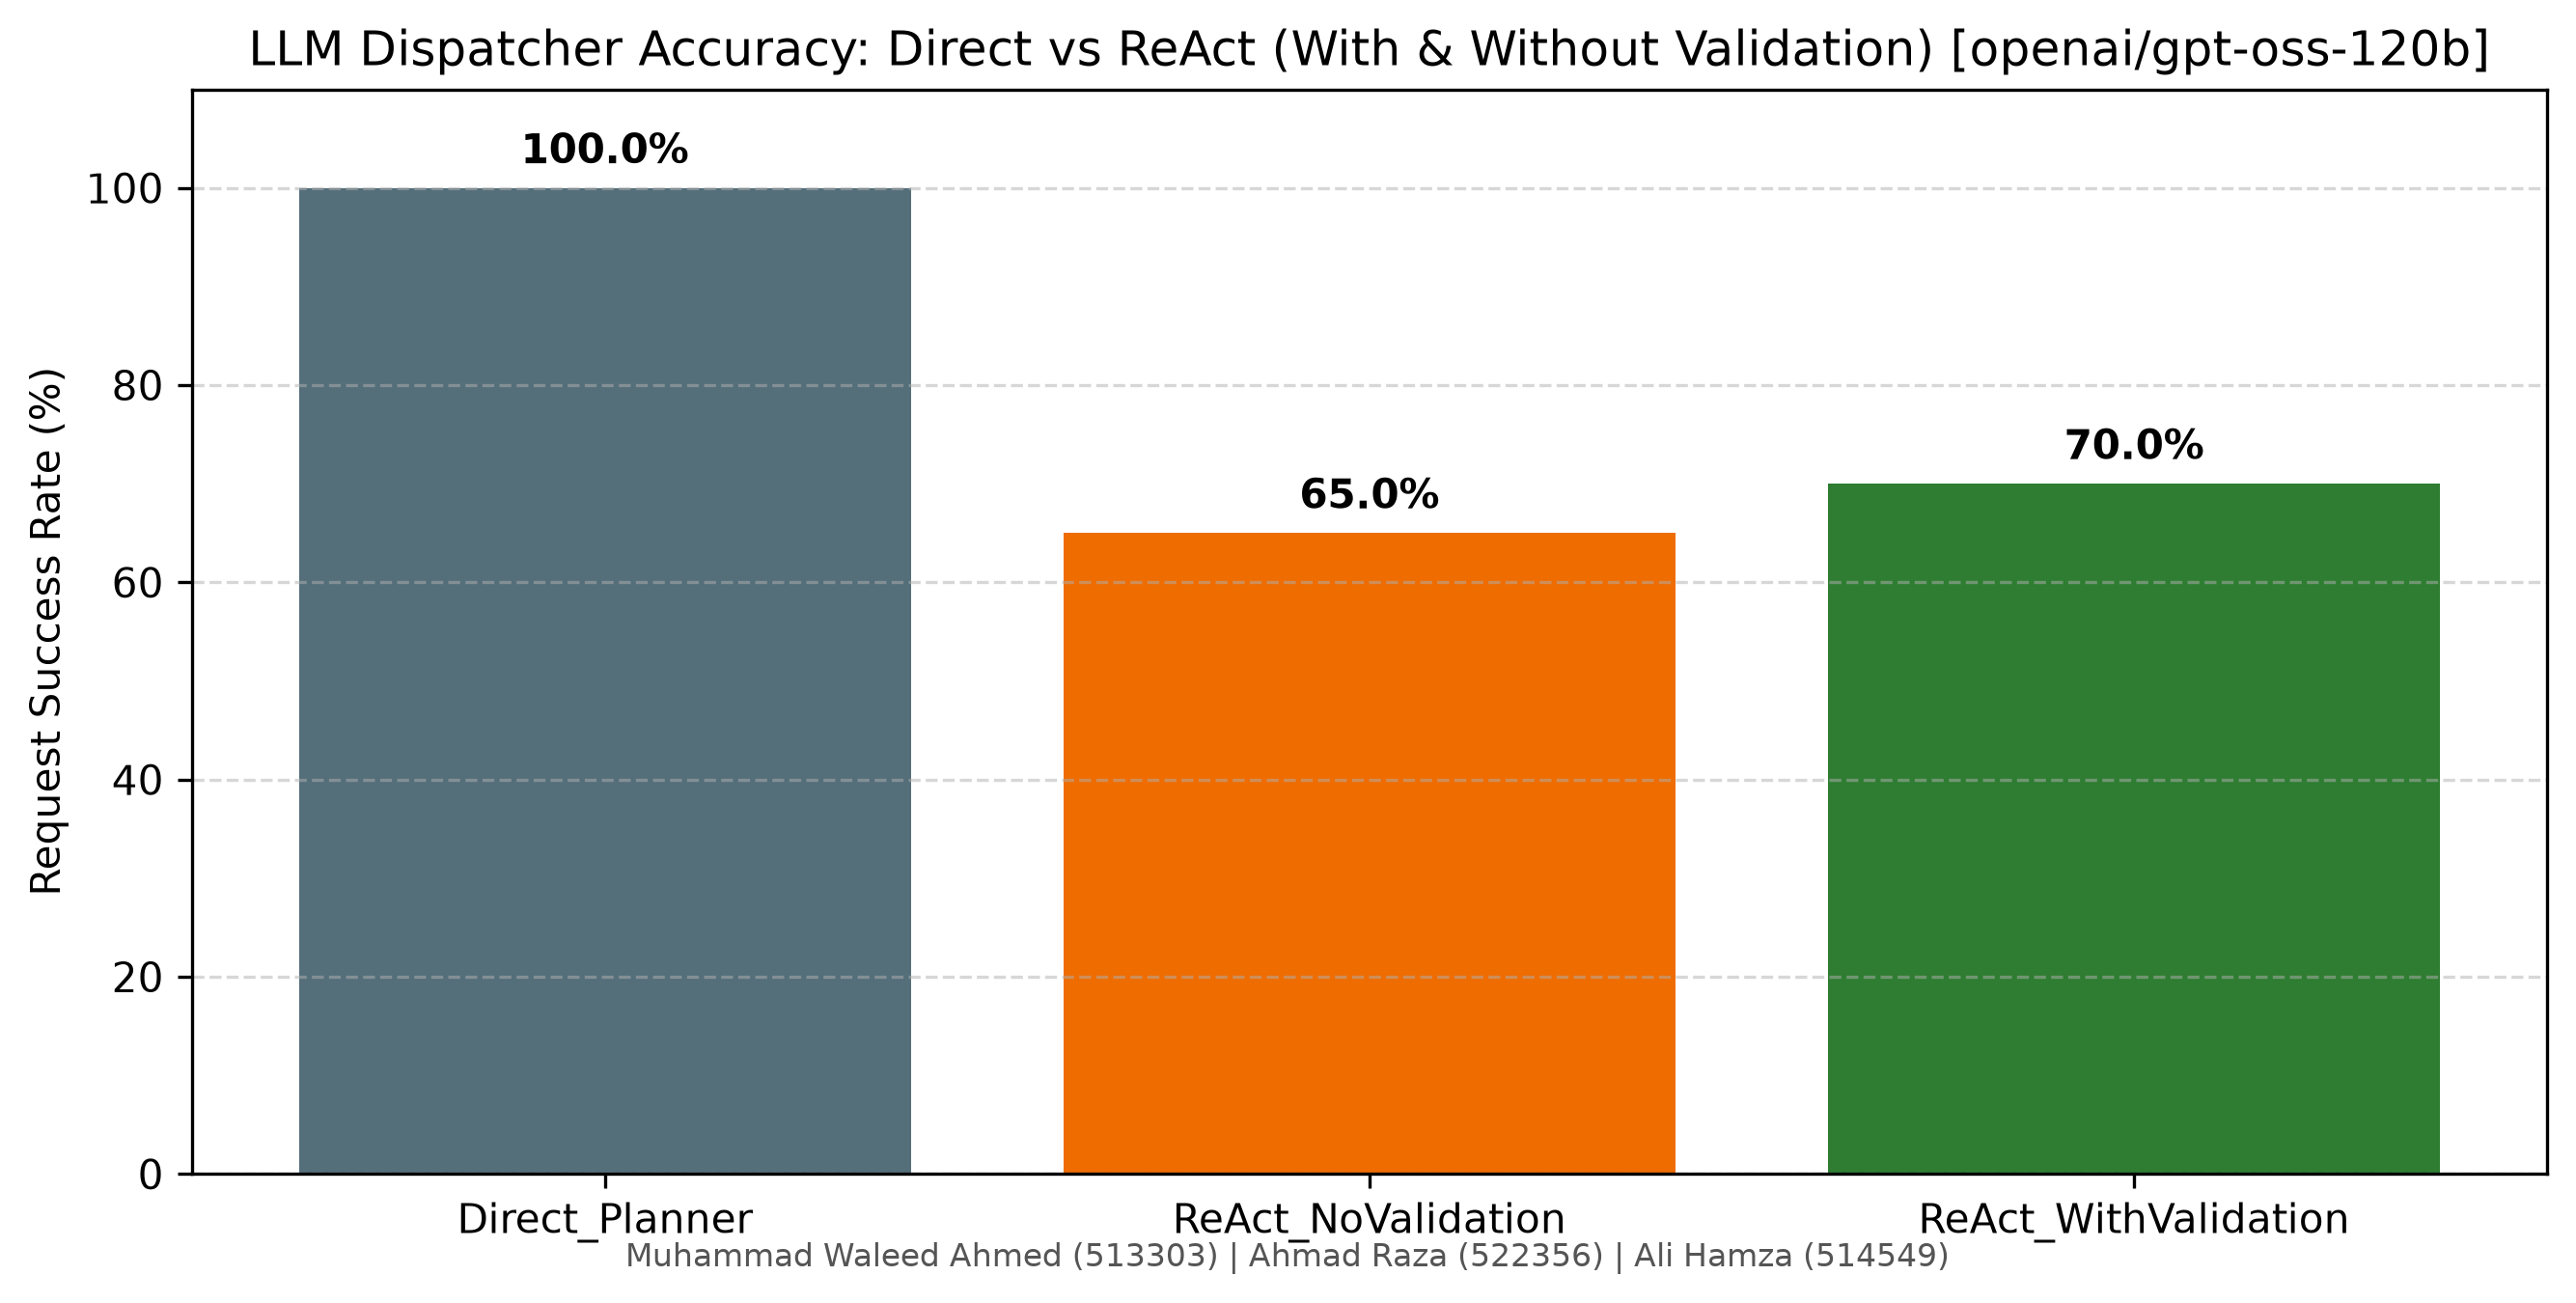
\includegraphics[width=0.90\columnwidth]{partD_llm_comparison.png}
    \caption{LLM dispatcher accuracy: Direct vs.\ ReAct with and without validation. | \stampline}
    \label{fig:partd}
\end{figure}

\texttt{ArgumentValidator} improved request success from \numPartdNovalSuccessPct{}\% to \numPartdWithvalSuccessPct{}\% and tool accuracy from $80.0\%$ to $85.0\%$. Observed live failures stemmed from Groq free-tier HTTP 429 rate limits/timeouts (\texttt{REQ-02/03/06/11/16}), malformed tool JSON schemas (\texttt{REQ-10/14}), and a premature stop after inspection (\texttt{REQ-09}). Table~\ref{tab:sra} maps representative traces to the Sense--Reason--Act cycle.

\begin{table}[t]
    \centering
    \caption{Sense--Reason--Act Mapping for Success, Rescue, and Failure Traces. | \stampline}
    \label{tab:sra}
    \scriptsize
    \begin{tabular}{@{}p{1.2cm}p{2.1cm}p{2.0cm}p{2.3cm}@{}}
        \toprule
        Trace & Sense & Reason Summary & Action / Gate \\
        \midrule
        \texttt{REQ-01} (Success) & Depot $(4,20)$, 5 stops, one-way/fog active & Inspect depot rules, plan A* (`own`), verify in sim & \texttt{inspect\_twists} $\rightarrow$ \texttt{plan\_route} ($C=268$) $\rightarrow$ \texttt{simulate} \\
        \texttt{REQ-19} (Rescue)  & Request forbids start $(4,20)$ & Attempt \texttt{plan\_route} with \texttt{forbidden\_cells=[[4,20]]} & \textbf{Blocked} by \texttt{ArgumentValidator}; returns \texttt{infeasible} \\
        \texttt{REQ-09} (Failure) & Request asks to inspect rules then plan & Inspect depot rules first & \texttt{inspect\_twists} $\rightarrow$ premature \texttt{FINAL\_ANSWER} (\texttt{plan:null}) \\
        \bottomrule
    \end{tabular}
\end{table}

\section{Ablation, Failure Analysis, and Interactive UI}
\textbf{Heuristic Ablation:} Across 30 paired scenarios (Table~\ref{tab:ablation}, Fig.~\ref{fig:ablation}), removing the MST term (B2 only) increases expansions from \numMNineAblationFullOwnExp{} to $3403.8$, while MST-Only expands \numMNineAblationMstOnlyExp{} nodes—confirming that the MST component provides the primary search-space reduction and the max with B2 tightens directed lower bounds.

\begin{table}[t]
    \centering
    \caption{Heuristic Component Ablation Across 30 Paired Scenarios. | \stampline}
    \label{tab:ablation}
    \scriptsize
    \begin{tabular}{@{}lrrr@{}}
        \toprule
        Configuration & Expansions (95\% CI) & Peak Stored & Time (s) \\
        \midrule
        1. B1 (Manhattan)    & 8316.5 [5083.0, 11550.0] & 8496.0 & 0.564 \\
        2. B2 (Max Directed) & 3403.8 [1859.2, 4948.4]  & 4054.4 & 0.243 \\
        3. MST-Only (Symm.)  & \numMNineAblationMstOnlyExp{} [199.5, 1592.0]   & 1204.7 & 0.084 \\
        4. Full Own (MST+B2) & \numMNineAblationFullOwnExp{} [195.9, 1588.6]   & 1198.8 & 0.088 \\
        \bottomrule
    \end{tabular}
\end{table}

\begin{figure}[t]
    \centering
    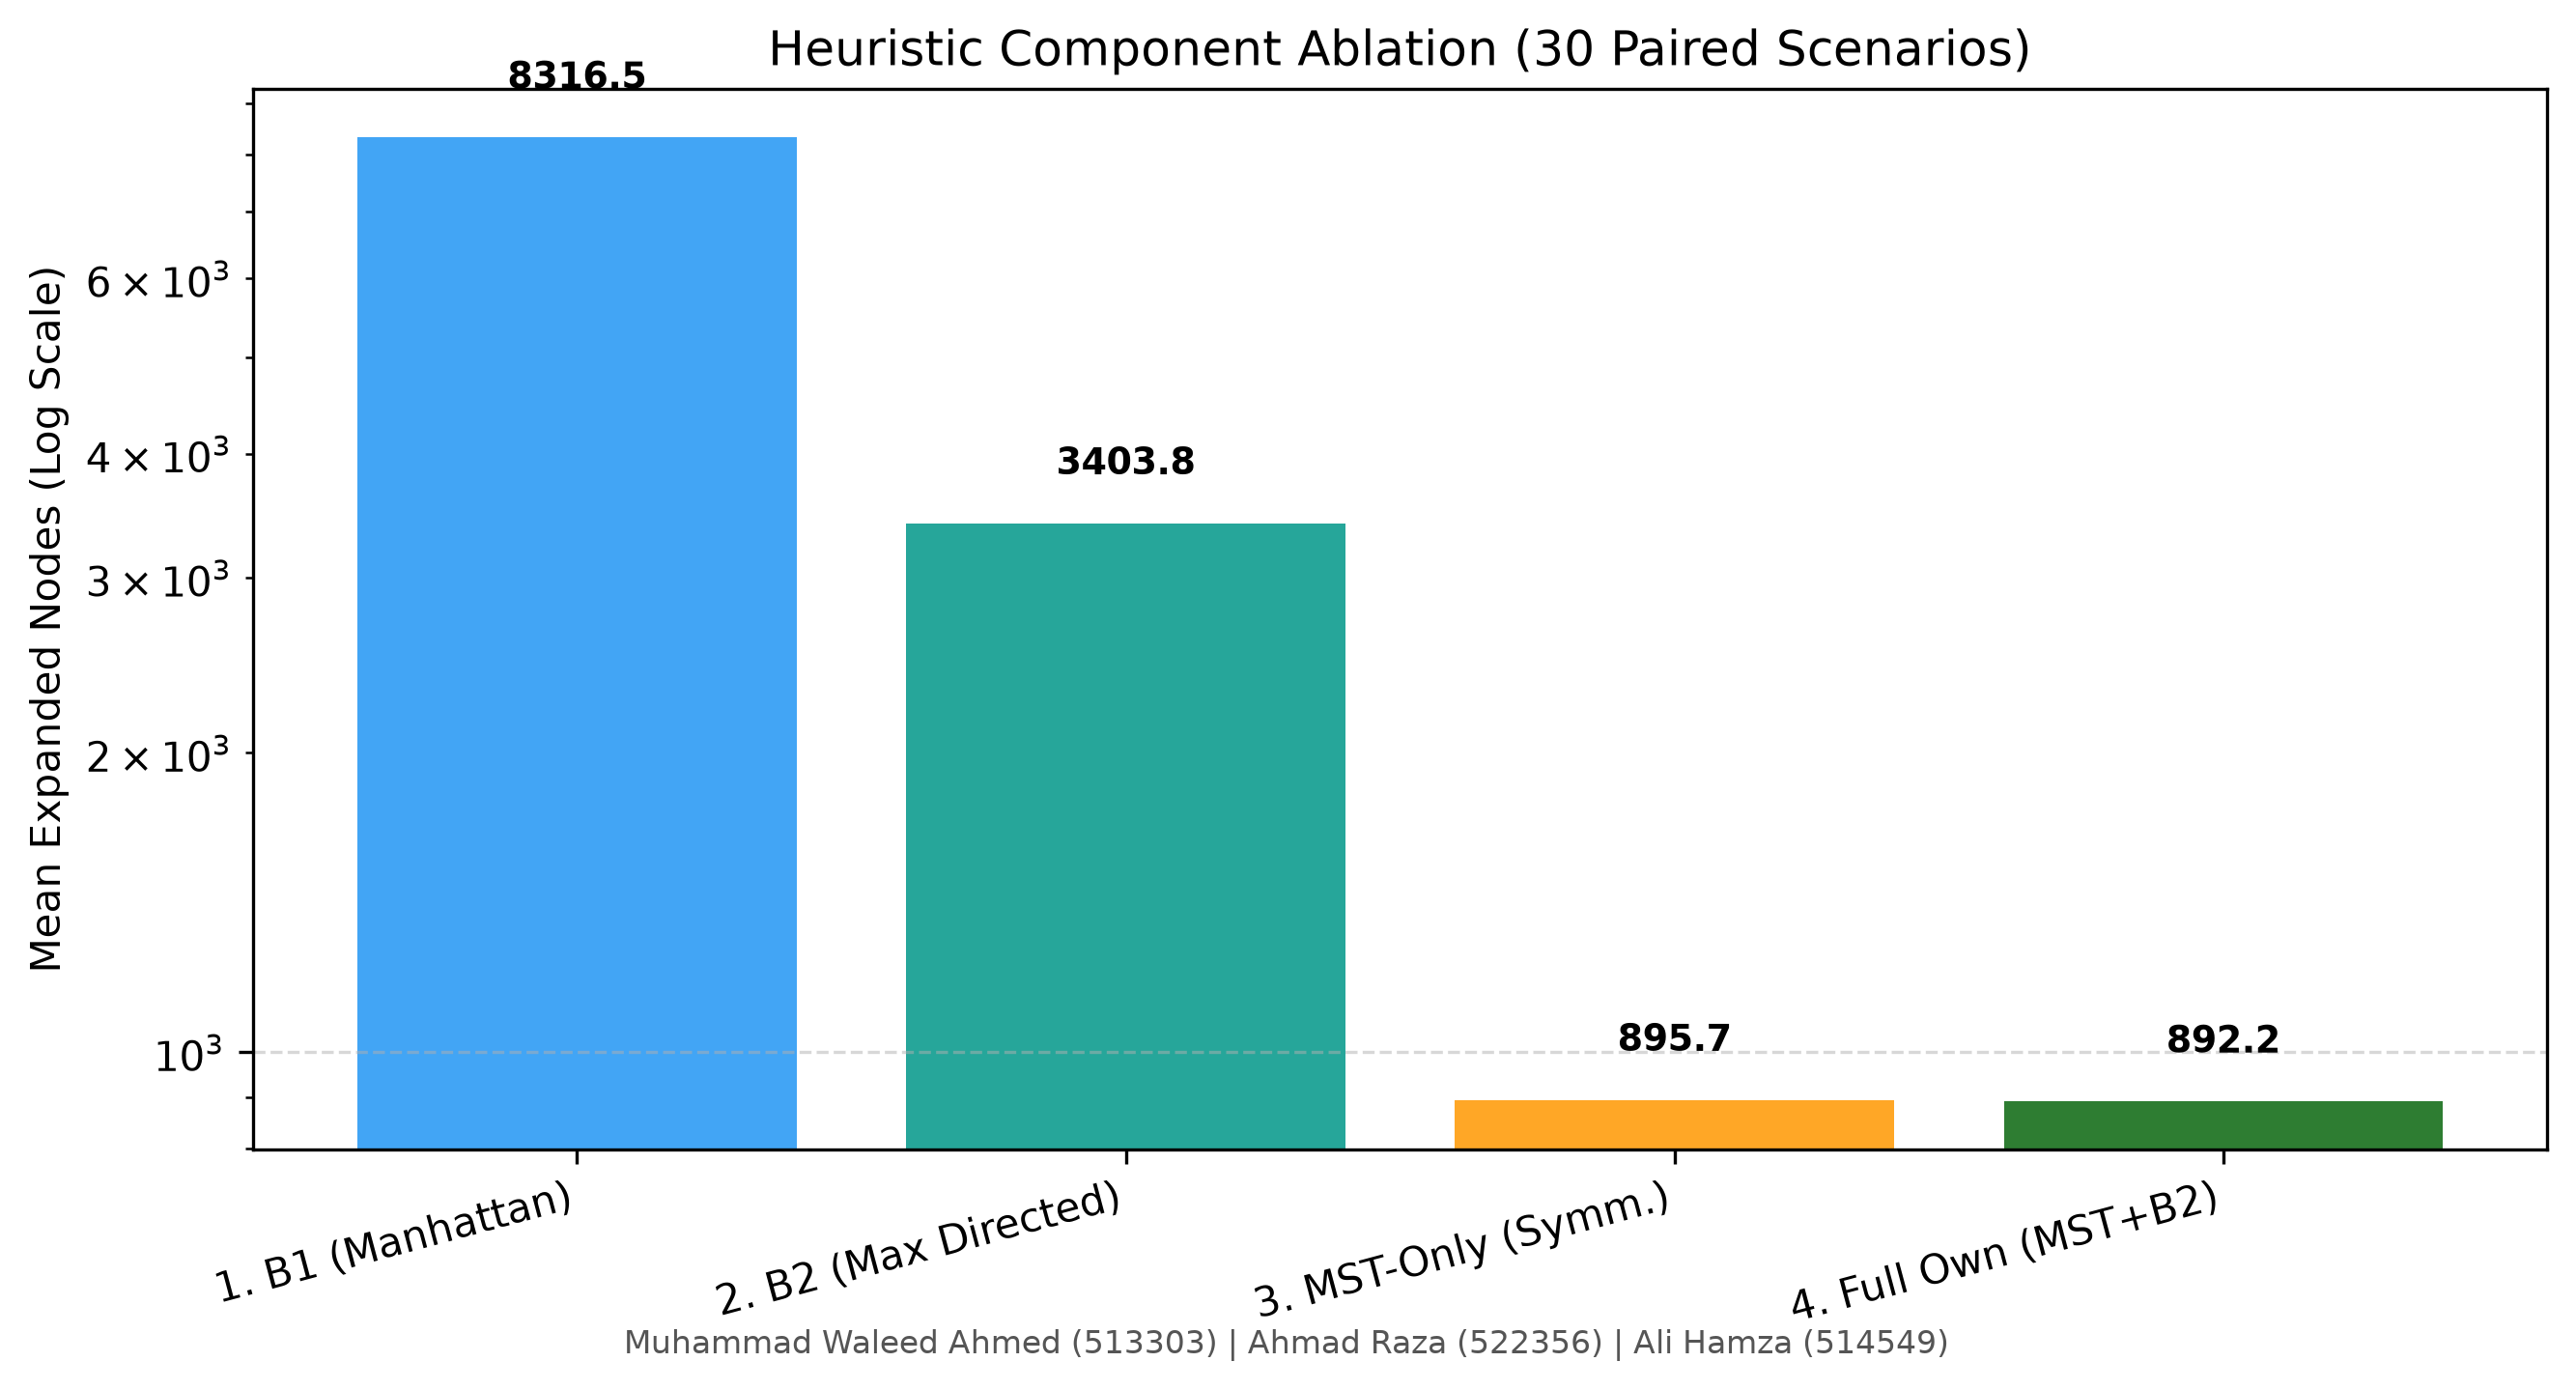
\includegraphics[width=0.90\columnwidth]{ablation_components.png}
    \caption{Ablation of heuristic components across 30 paired scenarios. | \stampline}
    \label{fig:ablation}
\end{figure}

\textbf{Cross-Stage Failure Analysis & UI:} Table~\ref{tab:failures} aggregates failures traced directly to raw experiment logs. Our 3-tab Streamlit UI (\texttt{delivery/ui/app.py}) exposes all validated planners, twist toggles, animated \texttt{chaser} games, and LLM dispatcher traces with persistent group stamping, and supports live-parameter reruns in $\sim 2.5$\,s.

\begin{table}[t]
    \centering
    \caption{Cross-Stage Failure Analysis Traced to Raw Logs. | \stampline}
    \label{tab:failures}
    \scriptsize
    \begin{tabular}{@{}p{2.3cm}rp{2.6cm}p{2.1cm}@{}}
        \toprule
        Category & Count & Root Cause & Mitigation \\
        \midrule
        Part A Reflex & 29/30 & Stateless local minima & Stateful A* planner \\
        Part B DLS/IDS & 90/210 & Depth/node cap DNF & A* + \texttt{CombinedMST} \\
        Part C Captures & 88/100 & Slip + \texttt{chaser} traps & Alpha-Beta + replan \\
        Part C Draws & 6/100 & Step/cost cap exhausted & Tuned route weights \\
        Part D Live LLM & 40/40* & HTTP 429/400 \& \texttt{REQ-09} & \texttt{ArgumentValidator} \\
        \bottomrule
    \end{tabular}
\end{table}

\section{Ethics, Reflection, and Conclusion}
\subsection{Ethical Impact and Implemented Safeguards}
Deploying autonomous delivery agents and LLM dispatchers affects parcel recipients (missed or misrouted deliveries), other road users (unsafe detours or one-way violations), couriers (unrealistic time/cost targets), and system operators. Concrete failure modes observed in our experiments include: (1) an LLM emitting an invalid or premature plan (\texttt{REQ-09}), (2) contradictory or hallucinated spatial arguments (\texttt{REQ-19}), (3) unmodelled stochastic slip pushing the agent into a rival capture, and (4) bounded-search cutoffs masquerading as infeasibility if not reported distinctly.

To mitigate these risks, our system implements five concrete safeguards: (1) \texttt{ArgumentValidator} blocks out-of-bounds, obstacle, and contradictory arguments prior to planner invocation; (2) a deterministic A* fallback and feasibility certificate (\texttt{FEASIBLE}/\texttt{INFEASIBLE}/\texttt{UNKNOWN}) separate resource limits from true unreachability; (3) hard expansion/time caps ($2\times 10^6$ nodes, $60$\,s) prevent runaway execution; (4) all LLM tool calls and simulator steps are logged in stamped audit traces; and (5) offline replay caching ensures reproducible auditing. Remaining limitations include deterministic lookahead under high slip ($p=0.5$), local $r=4$ window myopia in Part C, and hosted LLM rate-limit sensitivity.

\subsection{AI-Assistance Disclosure and Conclusion}
AI coding assistance was used for implementation scaffolding, test generation, and documentation formatting; all group members have reviewed the codebase and can explain every algorithm and line during the viva. Overall, combining a provably admissible MST-based heuristic, move-ordered Alpha-Beta pruning, slip-triggered replanning, and validated ReAct tool calling yields a reproducible, auditable autonomous delivery system.

\bibliographystyle{IEEEtran}
\bibliography{references}

\end{document}
